\documentclass[11pt,a4paper]{article}
\usepackage[utf8]{inputenc}
\usepackage{a4wide}
\usepackage{amsmath}
\usepackage{amsfonts}
\usepackage{amssymb}
\usepackage{graphicx}
\usepackage{float}
\usepackage{url}
\usepackage{amsmath}
%\usepackage[T1]{fontenc}
\usepackage{amsthm}
\usepackage{amssymb}
\usepackage[french,english]{babel}
\usepackage[babel=true,kerning=true]{microtype}
\usepackage[french]{cleveref}
\usepackage{svg}
\usepackage{caption}

\usepackage[left=3cm,right=3cm,top=3cm,bottom=3cm]{geometry}

\newtheorem{thm}{Theorem}
\newtheorem{prop}{Propriété}

\theoremstyle{definition}
\newtheorem{defn}{Définition}

\theoremstyle{remark}
\newtheorem{rmq}{Remarque}

\theoremstyle{remark}
\newtheorem{ex}{Exemple}

\def \stg {stream graph}
\def \Stgs {Stream graphs}
\def \Stg {Stream graph}
\def \stgm {stream graph multicouche}
\def \Stgm {Stream graph multicouches}
\def \stgs {stream graphs}
\def \stgms {stream graphs multicouches}
\def \Stgms {Stream graphs multicouches}


%tikz 
\usepackage{tikz}
\usepackage{pgfplots}
\usepackage{amsmath}
\usetikzlibrary{decorations.pathmorphing, positioning}
\definecolor{echoreg}{HTML}{2cb1e1}
\definecolor{echodrk}{HTML}{0099cc}
\tikzstyle{mybox} = [text=black, very thick,
    rectangle, rounded corners, inner sep=10pt, inner ysep=20pt]
\tikzstyle{fancytitle} =[text=black]
\newcommand{\yslant}{0.5}
\newcommand{\xslant}{-0.6}

%%%%%%%%%%%%%%%%%%%%%%%%%%%%%%%% TIKZ STYLES
\tikzstyle{every node}=[font=\scriptsize]

\tikzset{RootStyle/.style = {
						shape          = circle,
			      draw           = red!50!black!50,
			      thick,
			      top color      = white,
			      bottom color   = red!50!black!20,
			      text           = black,
			      inner sep      = .2pt,
			      outer sep      = 0pt,
			      minimum size   = 2.5 mm}
						}

\tikzset{VertexStyle/.style = {
						shape          = circle,
			      draw           = black!50,
			      top color      = white,
			      bottom color   = black!20,
			      text           = black,
			      inner sep      = .2pt,
			      outer sep      = 0pt,
			      minimum size   = 1.75 mm}
						}

\tikzset{EdgeStyle/.style   = {thick,<->}}

\tikzset{LabelStyle/.style =   {
				  text           = black,
				  inner sep      = .2pt,
				  outer sep      = 1pt,
				  font           =\scriptsize,
				  minimum size   = 2.15 mm}
					}

\pgfplotsset{compat=1.15}

\newcommand\overmat[3]{%
  \makebox[0pt][l]{$\smash{\color{#3}\overbrace{\phantom{%
    \begin{matrix}#2\end{matrix}}}^{\text{#1}}}$}#2}
\newcommand\undermat[3]{%
  \makebox[0pt][l]{$\smash{\color{#3}\underbrace{\phantom{%
    \begin{matrix}#2\end{matrix}}}_{\text{#1}}}$}#2}
\newcommand\partialphantom{\vphantom{\frac{\partial e_{P,M}}{\partial w_{1,1}}}}

\author{Pimprenelle Parmentier}



\title{Stream graphes multicouches}
\begin{document}
\selectlanguage{french}
\begin{titlepage}


\noindent
\textsc{Ecole polytechnique}\\
PROMOTION X2016 \\
MASTER: Mathématiques appliquées\\
PARMENTIER Pimprenelle

\vspace{3cm}
\begin{center}
\textsc{\Large Rapport de stage}
\vspace{1cm}
\hrule % Horizontal line
\vspace{0.4cm}
{\huge \bfseries \Stgms \par}\vspace{0.4cm} % Thesis title
\hrule 
\vspace{1cm}
\textsc{\Large Rapport non confidentiel}
\vspace{4cm} % Horizontal line
 
\end{center}

\noindent
\textit{Option:} Mathématiques appliquées\\
\textit{Champ:} Recherche opérationnelle, théorie des graphes\\
\textit{Enseignant référent:} Xavier \textsc{Allamigeon}\\
\textit{Tuteur de stage dans l'organisme:} Tiphaine \textsc{Viard}\\
\textit {Co-tuteurs de stage hors organisme:} Benjamin \textsc{Renoust} (Université d'Osaka)\\
\hspace*{3.1cm} Jean-François \textsc{Baffier} (Japan Society for the Promotion of Science)\\
\textit{Dates du stage:} 8 avril 2019 - 23 aout 2019\\
\textit{Adresse de l'organisme:}\\
RIKEN AIP\\
Nihonbashi 1-chome Mitsui,\\
Building, 15th floor,\\
1-4-1 Nihonbashi,\\
Chuo-ku, Tokyo\\
103-0027, Japan\\
\end{titlepage}


\begin{abstract}

Ce rapport de stage traite d'un nouvel objet permettant de traiter de graphes complexes dépendants du temps : les \textbf{\stgms{}}. 

Dans un premier lieu, nous ferons un état de l'art sur les formalismes existant pour traiter de graphes complexes et de graphes temporels. Nous présenterons ainsi les graphes multicouches et les \stgs{} qui nous servirons à construire les \stgms{}. 

Dans un second temps, nous donnerons une définition formelle des \stgms{}, et nous montrerons en quoi ce nouvel objet est une généralisation des objets existants. Puis nous définirons des mesures permettant d'étudier les \stgms{}, qui prennent en compte l'aspect à la fois multicouche et temporel.

Nous présenterons ensuite la bibliothèque python concue pour traiter ce type d'objet, ainsi qu'un exemple d'utilisation avec un jeu de données temporel multicouche.

Enfin, nous donnerons un ensemble de pistes que nous pourrons explorer pour la suite du stage.

\end{abstract}

\selectlanguage{english}

\begin{abstract}

\end{abstract}

\selectlanguage{french}

\newpage 

\tableofcontents
\newpage


\section*{Remerciements}

    En premier lieu, je souhaite remercier ma tutrice Tiphaine \textsc{Viard}, qui a rendu mon stage possible, ainsi que mes co-tuteurs Jean-François \textsc{Baffier} et Benjamin \textsc{Renoust} pour leur accompagnement pendant la durée du stage. Grâce à leurs conseils et leur suivi, j'ai pu apprendre beaucoup de choses dans le domaine des graphes mais également sur la recherche en général.
    
    Je remercie également les équipes administratives de Riken et de l'Ecole Polytechnique pour leur support.

\newpage

\section*{Introduction}
	Le concept de graphe remonterait à Euler \cite{wikigraphes,divin} dans les années 1750, qui énonça le problème des ponts de Königsberg. Cet objet s'est par la suite révélé extrêmement puissant pour résoudre de nombreux problèmes en algorithmique, en probabilités, en combinatoire, en optimisation et plus récemment pour traiter des données. Les graphes sont utilisés dans de nombreux domaines appliqués, que ce soit en informatique (analyse de réseaux sociaux, PageRanking \cite{pr}), en biologie, ou dans l'étude des transports par exemple.
	
	La puissance de la théorie des graphes vient du fait qu'elle permet d'exprimer des problèmes réels variés dans un même formalisme très simple, pour lequel des algorithmes ont été créés.
	
	Cependant, une partie de l'information est alors perdue, notamment le fait que les interactions entre différents individus dépendent souvent du temps. On "lisse" volontairement les différences au sein des noeuds et des liens, mais une fois encore, on simplifie beaucoup la représentations de nos données. C'est cette \og simplification \fg{}  qui permet de synthétiser un problème pour y trouver des solutions, mais il pourrait être intéressant de créer un objet plus complexe pour traiter de nouveaux problèmes moins adaptés au formalisme des graphes.
	
	Notre objectif ici est, en partant de formalismes déjà construits, de créer un nouvel objet nous permettant de représenter des graphes dépendant du temps et prenant en compte les différences au sein des noeuds et des liens : nous appellerons cet objet le \stgm. Dans une première partie, nous établirons un état de l'art en rappelant les définitions des graphes, des graphes multicouches et des \stgs{}, nous donnerons une bibliographie associée et une analyse critique de ces formalismes. 
	
	Ensuite, nous présenterons notre nouvel objet, le \og \stgm{} \fg{} , les définitions associées. Nous expliquerons comment retrouver les graphes \og classiques\fg{} à partir de ce nouvel objet, grâce à diverses projections.
	
	Nous présenterons enfin la bibliothèque que nous avons créée pour étudier les \stgms{} ainsi que quelques exemples de bases de données pour lesquelles il est judicieux d'utiliser notre outil et les résultats que nous avons obtenus sur ces bases. 
	
	En dernier lieu, nous parlerons des perspectives que ce formalisme ouvre et de nos pistes dans le futur.
	
	
	
\section{Etat de l'art : deux formalismes sur les graphes}
\indent

Dans cette partie, nous allons présenter les objets qui ont servi à construire les \stgms{} : tout d'abord les \textbf{graphes}, puis les \textbf{graphes multicouches} qui servent à différentier les noeuds et les arêtes, et les \textbf{\stg{}} qui permettent de modéliser des graphes dépendant du temps.

\subsection{Les graphes}

\begin{defn}[Graphe]
Un graphe $G$ est un ensemble de n\oe{}uds $V$ ainsi qu'un ensemble d'arêtes $E$, chaque element de $E$ étant une paire non ordonnée de deux éléments de $V$. Les arêtes représentent une interaction entre deux n\oe{}uds.
\end{defn}

Nous avons donné ici la version la plus simple des graphes, mais il existe de nombreuses variantes, comme les graphes orientés, les graphes pondérés ou les graphes colorés, entre autres.

\begin{defn}[Paires ordonnées et non ordonnées]
	$A$ et $B$ sont deux ensembles non vides.
	
	On appelle ensemble des \textit{paires ordonnées} de $A$ et $B$ l'ensemble $\{ (a,b) | a \in A \text{ et } b \in B\}$. L'ensemble est appelé $A \times B$.
	
	On appelle ensemble des \textit{paires non ordonnées} de $A$ et $B$ l'ensemble $\{(u,v) | u \in A \text{ et } v\in B \textbf{ ou } u \in B \text{ et } v\in A\}$. L'ensemble est appelé $A\otimes B$.
\end{defn}

	Les paires ordonnées servent à représenter des graphes orientés tandis que les paires non ordonnées servent à représenter des graphes non ordonnées.

\begin{figure}[h]
			\begin{center}
					\begin{tikzpicture}[xscale=2,yscale=2,auto]
							\draw (2,0) node[VertexStyle]   (A) { A };
							\draw (0,0) node[VertexStyle] (B) { B };
							\draw (0,2) node[VertexStyle]   (C) { C };
							\draw (2,2) node[VertexStyle]   (D) { D };

							\draw[EdgeStyle]				(B) to node[LabelStyle]{}	(A);
							\draw[EdgeStyle,bend left=40,looseness=1.1]    	(C) to node[LabelStyle]{}   	(A);
							\draw[EdgeStyle] 	(C) to node[LabelStyle]{}     	(B);
							\draw[EdgeStyle]  	(C) to node[LabelStyle]{} 		(D);
							

					\end{tikzpicture}
			\end{center}
	\caption{Un exemple de graphe d'interaction, par exemple entre divers individus de la même espèce. Un lien existe entre deux animaux s'ils ont été en contact.}
	\label{fig:tikzminimal}
\end{figure}


Comme dit en introduction, la théorie des graphes permet de modéliser et de résoudre de nombreux problèmes de la vie réelle, en synthétisant des informations. Ces problèmes sont étudiés depuis plus de 200 ans et nous avons à présent de nombreux outils pour les étudier, même si le domaine est encore en évolution.

\subsection{Les graphes multicouches}

Les graphes permettent de synthétiser et de représenter des interactions entre individus. Nous choisissons donc de ne représenter qu'un seul type de relations entre un seul type d'individus, soit en ignorant leurs différences, soit en ne représentant qu'une partie des relations et des noeuds. 

Pour pallier à cette \og approximation\fg{}, l'objet graphe multicouche a été créé.

\subsubsection{Définition générale}

 Les graphes multicouches sont utilisés pour décrire des interactions entre des noeuds qui peuvent être de différentes natures de façon simultanée et/ou qui peuvent avoir des interactions de natures différentes. 
 
 Une définition très générale des graphes multicouches est donnée dans le papier \cite{mlkiv}, nous la résumons ici.
 
 \begin{defn}{Graphe multicouche}
 
 La structure d'un graphe multicouches est décrite par le k-uplet d'ensembles ${\cal L} = L_1, \dots , L_k$. Chaque $L_i$, appelé {\em aspect}, est un ensemble d'attributs, appelés {\em couches élémentaires}. Chaque {\em couche} correspond à un élément de $L=L_1\times L_2 \times \dots \times L_k$.
 
 Un graphe multicouches s'écrit alors $M = (V_M, E_M, V, L)$. $V$ est l'ensemble de ses {\em noeuds}, $L$ la {\em structure} des couches, $V_M$ sont les {\em noeuds-couches}, qui comme leur nom l'indique, sont les éléments de $V\times L$. Enfin $E_M \subseteq V_M \times V_M $ est l'ensemble des {\em arêtes}, une arête pouvant relier deux noeuds-couches entre eux. 

	\end{defn}
 
 On peut trouver un exemple de graphe multicouche \cref{exmulti}.

\begin{figure}[h]
	\centering
	
%0.58
\begin{tikzpicture}[scale=0.38,every node/.style={minimum size=1cm},on grid]

	\node [mybox, scale=1.0] at (10.5, 2) (box){%
		\begin{minipage}{0.6\textwidth}
			
    	\end{minipage}
	};
	
	
	% etage 2
	\begin{scope}[
		yshift=-210,
		every node/.append style={yslant=\yslant,xslant=\xslant},
		yslant=\yslant,xslant=\xslant
	] 
		%\draw[black, dashed, thin] (0,0) rectangle (7,7); 
		\fill[olive,fill opacity=.75] (0,0) rectangle (7,7);
		
		\fill[orange,fill opacity=.75] (10,0) rectangle (17,7);
		%\draw[black, dashed, thin] (10,0) rectangle (17,7); 
		
		\draw[fill=echoreg]  %foret, collabo
			(5,2) node(111){} circle (.1) %A
			(2,2) circle (.1) %B
			(2,5) circle (.1); %C
			%(5,5) circle (.1); %D
		
		\draw[fill=echoreg]  %plaine, collabo
			(15,2) node(111){} circle (.1) %A
			%(12,2) circle (.1) %B
			(12,5) circle (.1) %C
			(15,5) circle (.1); %D
		 
		\draw[ thin, color=echodrk]%foret collab
			(2,4.9) to (2,2.1); %C->B
		\draw[ thin, color=echodrk]
			(2.1,2) to (4.9,2);%B->A
		
		\draw[thin, color=echodrk]%plaine collab
			(12,5) to (15,2);%C->A
		\draw[thin, color=echodrk]
			(12,5) to (15,5);
			
		\fill[black]
			(0.5,6.5) node[right, scale=.7] {Forêt, Collaboration}	
			(5.1,1.9) node[right,scale=.7]{\bf A}
			(1.9,1.9) node[left,scale=.7]{\bf B}
			(2,5.2) node[left,scale=.7]{\bf C};
			%(5.2,5.1) node[right,scale=.7]{\bf D}; 
			
		\fill[black]
			(10.5,6.5) node[right, scale=.7] {Plaine, Collaboration}	
			(15.1,1.9) node[right,scale=.7]{\bf A}
			%(11.9,1.9) node[left,scale=.7]{\bf B}
			(12,5.2) node[left,scale=.7]{\bf C}
			(15.2,5.1) node[right,scale=.7]{\bf D}; 
		
		
	\end{scope}
	
	% Interlayer crossconnections
	% vertical
	\draw[thick,  dashed, decorate] (3.8, 4) to (3.8, -3.5);%A
	\draw[thick, dashed, decorate] (.8,2.4) to (.8,-5);%B
	\draw[thick,  dashed, decorate] (-1, 4.5) to (-1, -2.8);%C
	
1	\draw[thick,  dashed, decorate] (13.8,9) to (13.8, 1.5);%A
	\draw[thick, dashed, decorate] (12,11) to (12,3.6);%D
	\draw[thick,  dashed, decorate] (9, 9.5) to (9, 2.1);%c
	
	%horizontal
	
	
	\draw[thick, dashed, decorate] (-1,-2.8) to[bend left] (9,2.1);
	\draw[thick, dashed, decorate] (3.8,-3.5) to[bend left] (13.8,1.5);
	
	
	% etage 1
	\begin{scope}[
		yshift=0,
		every node/.append style={yslant=\yslant,xslant=\xslant},
		yslant=\yslant,xslant=\xslant
	]
		\fill[olive,fill opacity=.85] (0,0) rectangle (7,7); 
		%\draw[black, dashed, thin] (0,0) rectangle (7,7); 
		
		\fill[orange,fill opacity=.85] (10,0) rectangle (17,7);
		%\draw[black, dashed, thin] (10,0) rectangle (17,7); 
		
		\draw [fill=red]
			(5,2) node(111){} circle (.1)%A %foret, combat
			(2,2) circle (.1)%B
			(2,5) circle (.1)%C
			(5,5) circle (.1);%D

		\draw[fill=red]  
			(15,2) node(111){} circle (.1) %A % plaine combat
			%(12,2) circle (.1) %B
			(12,5) circle (.1) %C
			(15,5) circle (.1); %D
		
		\draw[thin, color=red]%foret combat
			(2,2.1) to (2,4.9);%B->C
			
		\draw[thin, color=red]%plaine combat
			(12,5) to (15,5);%C->D
		
		
		\fill[black]
			(0.5,6.5) node[right, scale=.7] {Forêt, Combat}
			(5.1,1.9) node[right,scale=.7]{\bf A}
			(1.9,1.9) node[left,scale=.7]{\bf B}
			(1.9,5) node[left,scale=.7]{\bf C}
			(5.2,5.1) node[right,scale=.7]{\bf D}; 
			
		\fill[black]
			(10.5,6.5) node[right, scale=.7] {Plaine, Combat}
			(15.1,1.9) node[right,scale=.7]{\bf A}
			%(11.9,1.9) node[left,scale=.7]{\bf B}
			(12,5.2) node[left,scale=.7]{\bf C}
			(15.2,5.1) node[right,scale=.7]{\bf D};
			
	\end{scope} 
	
	%interlayer
	\draw[thick, dashed, decorate] (-1,4.5) to[bend left] (9,9.5);
	\draw[thick, dashed, decorate] (3.8,4) to[bend left] (13.8,9);
	\draw[thick, dashed, decorate] (2.1,6.1) to[bend left] (12,11);
\end{tikzpicture}

	\caption{\textbf{Représentation d'un graphe multicouches.} Ici, les noeuds sont des animaux d'une même espèce représentés par leurs initiales: $V = \{A ,B,C,D \}$. Chaque couche est caractérisée par une milieu naturel et un type de relation: $L = \{$Milieu, type de relation$\}$. Les noeuds couches existent ou non en fonction de la présence ou non d'un animal dans un milieu pour un type de relation: $V_M$ contient par exemple (A;Forêt,Combat). Enfin, les liens représentent les interaction entre les animaux dans un milieu précises: $E_M$ contient par exemple ((B;Forêt,Collaboration),(C;Forêt, Collaboration)).}
	\label{exmulti}
\end{figure}

\subsubsection{Cadres d'utilisation}


Les graphes multicouches trouvent de nombreuses applications, par exemple en \textbf{écologie} \cite{ecolo} (les noeuds sont alors des espèces ou des individus, les couches élémentaires des types d'interaction (parasite, prédateur...), des lieux, des temps, etc. On cherche alors à savoir comment se diffuse une maladie, quelles sont les faiblesses d'un écosystèmes (quels sont les liens / nœuds qui assurent le bon fonctionnement ?)

Un autre jeu de données utilisé est en \textbf{économie}, celui des interactions entre les banques européennes \cite{interbank}, les couches étant caractérisées par le type d'interaction (de "prêt"), les noeuds étant les banques et un lien existant entre deux banques de la même couche quand celles-ci procèdent à une interaction du type correspondant.

Un dernier exemple intuitif est celui des \textbf{réseaux de transport}, dans lequel les couches sont les différents moyens de transport possible, les nœuds sont des localités et les liens les différentes lignes de transport. Un tel jeu de données peut être trouvé sur le site gouvernemental américain des statistiques de transport, pour les lignes aériennes \cite{plane}.

On remarque que dans beaucoup de situations, nous avons des liens "implicites" entre tous les différents noeuds-couches issus du même noeud, et des liens "explicites" ne pouvant apparaitre qu'au sein d'une même couche. De tels graphes sont appelés \textbf{multiplexes}.





%Ils permettent de représenter des graphes de collaboration entre chercheurs par exemple : chaque chercheur collabore avec d'autres sur des mots-cles précis, les noeuds sont alors les chercheurs, les couches les différents mots-clés utilisés et des liens apparaissent entre deux chercheurs-mots clés quand les deux chercheurs apparaissent sur le même papier traitant du mot-clé.

\subsubsection{Quelques définitions}

\begin{defn}{\textbf{Tenseur d'adjacence}}
	
\end{defn}
D'un point de vue pratique, ces graphes peuvent être manipulés à l'aide de tenseurs d'adjacence \cite{mldd}, d'ordre 4. Chaque élément $M^{u,\alpha}_{v,\beta}$ indique s'il existe un lien entre les nœuds-couches $(u,\alpha)$ et $(v,\beta)$.

\begin{defn}{\textbf{Arêtes intra-couches et inter-couches.}}
	On appelle arêtes inter-couches les arêtes qui lient deux nœud-couches de couches différentes. (L'ensemble des arêtes inter-couches s'écrit $E_A = \{((u,\alpha),(v,\beta)) \in E_M | \alpha = \beta\}$). On appelle arêtes intra-couches les arêtes qui lient deux noeuds-couches de la même couche. (L'ensemble correspondant s'écrit $E_C = E_M\backslash E_A$).
\end{defn}
Ainsi, les multiplexes sont des graphes multicouches dans lesquels les seuls arêtes intercouches autorisées sont les arêtes entre les noeuds-couches du même noeud.

\begin{defn}{\textbf{Graphe agrégé}}
	On appelle le graphe aggrégé le graphe qu'on obtient en "superposant" les couches d'un graphe multicouches : $$G=(V_G,E_G), \quad V_G=V, \quad E_G={(u,v)|\exists \alpha, \beta | ((u,\alpha),(v,\beta)) \in E_M}$$.
\end{defn}

\begin{defn}{\textbf{Graphe sous-jacent}}
Le graphe sous-jacent de $M$ est le graphe qu'on obtient en faisant abstraction de la structure multicouches, et dans lequel chaque noeud est un noeud-couche.
$$G=(V_{SJ},E_{SJ}), \quad V_{SJ} = V_M, \quad E_{SJ}=E_M$$
\end{defn}




\subsubsection{Pourquoi utiliser des graphes multicouches à la place de graphes classiques ?}

On remarque que dans beaucoup de cas, les graphes sont des graphes agrégés ou sous-jacent de graphes multicouches. Une partie de l'information a été "perdue" mais cela permet d'utiliser des outils très puissants et d'obtenir des résultats déjà satisfaisants grâce à la théorie des graphes. On peut donc se demander quel est l'intérêt d'utiliser ce formalisme, et de garder une telle quantité d'informations. De nouvelles mesures et de nouveaux algorithmes ont donc été créés pour pouvoir analyser plus finement ces informations plus détaillées.

En voici deux exemple, qui seront source d'inspiration dans la suite sur ce qu'il sera possible de faire avec l'objet que nous allons introduire.


\paragraph{Importance de la structure : Isomorphismes de graphes}

Deux graphes $G_1$ et $G_2$ sont dits isomorphes quand on peut trouver une bijection des sommets du premier graphes vers ceux du second qui préserve les arêtes.


\begin{figure}[H]
\centering
	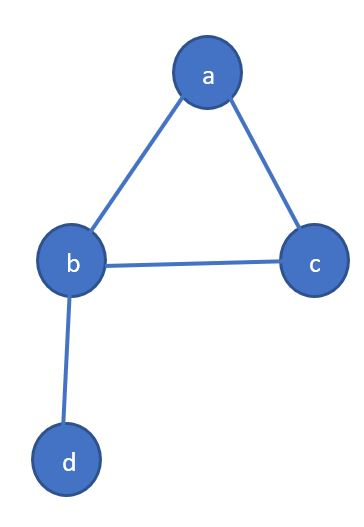
\includegraphics[width=0.2\textwidth]{graph1iso.JPG}
	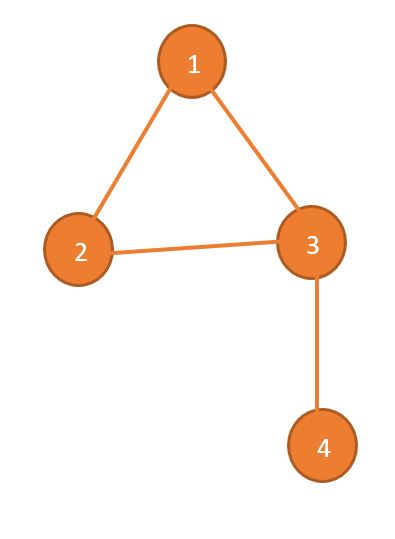
\includegraphics[width=0.2\textwidth]{graph2iso.JPG} 
	
	\caption{Un exemple de deux graphes isomorphes : $\sigma(a)=1, \sigma(b)=3, \sigma(c)=2, \sigma(d)=4$}
\end{figure}

Dans le cadre des multicouches, Kivelä et Porter \cite{isoMulti} définissent l'automorphisme de graphe (sans perte de généralité) par une permutation des arêtes, des couches élémentaires et des couches qui préserve les liens.


Kiveä et Porter démontrent qu'il n'est pas équivalent de dire que deux graphes multicouches sont isomorphes et leurs graphes sous-jacent sont équivalents. En effet, il ne faut pas perdre de vue que la structure \og arborescente \fg{} des couches, doit être conservée, et pas seulement l'idée de \og partition \fg{} des nœuds en différentes couches. Ils présentent un algorithme permettant de vérifier si deux graphes multicouches sont isomorphes.

\paragraph{Centralité}

La question de la centralité a été traitée dans \cite{centraliteMulti}. De Domenico met en avant le fait qu'il est "réducteur" de calculer des centralités sur des graphes agrégés pour trouver quels sont les noeuds ayant les roles les plus centraux dans la cohésion de l'ensemble d'une structure. Ils définissent donc un nouveau "PageRank" et une nouvelle centralité intermédiaire (betweeness centrality). Le PageRank est calculé à partir du tenseur d'adjacence du graphe, on obtient alors des centralités pour chaque noeud-couche, qu'on traite de la manière la plus adaptée en fonction du problème à résoudre.

La centralité intermédiaire est calculée en sommant les centralités intermédiaires des différents nœuds-couches.

De Domenico montre que le fait de conserver l'information multicouche permet de trouver un classement des noeuds en fonction de leur centralité plus proche de la réalité (il compare ses résultat avec des données réelles sur les aéroports par exemple).

\paragraph{}

Nous avons présenté ici deux exemples pour lesquels il a été judicieux de conserver l'aspect mutlicouche des graphes, parce qu'il contient plus d'informations, et qu'elles ont une structure particulière. Nous avons également montré comment contruire des graphes \og classiques \fg{} à partir de projections sur graphes multicouches, et donc que les graphes multicouches sont une généralisation des graphes.


\subsection{Les \stgs }

Nous présentons maintenant un autre outil récemment créé permettant de traiter de la temporalité dans les graphes : les \stgs .
\subsubsection{Définition}

\begin{defn}{\textbf{\Stg}}
Un \stg{} s'écrit $S=(T,W,V,E)$. $T$ représente l'intervalle de temps d'étude de notre graphe. $V$ est l'ensemble des nœuds, et $W \subseteq T \times V$ est l'ensemble des nœuds de $V$ apparaissant en fonction du temps. Enfin, $E \subseteq T \times V \times V$ est l'ensemble des arêtes dont l'existence dépend également du temps. Étant donné un nœud $u$, on appelle $T_u$ l'union des intervalles pendant lesquels $u$ apparait, de même que $T_{u,v}$ décrit les temps d'apparition du lien $(u,v)$.
\end{defn}

La représentation graphique des \stgs{} est une des grandes forces du concept et permet de visualiser l'évolution des graphes au fil du temps avec une représentation statique.

\begin{figure}[H]
\centering
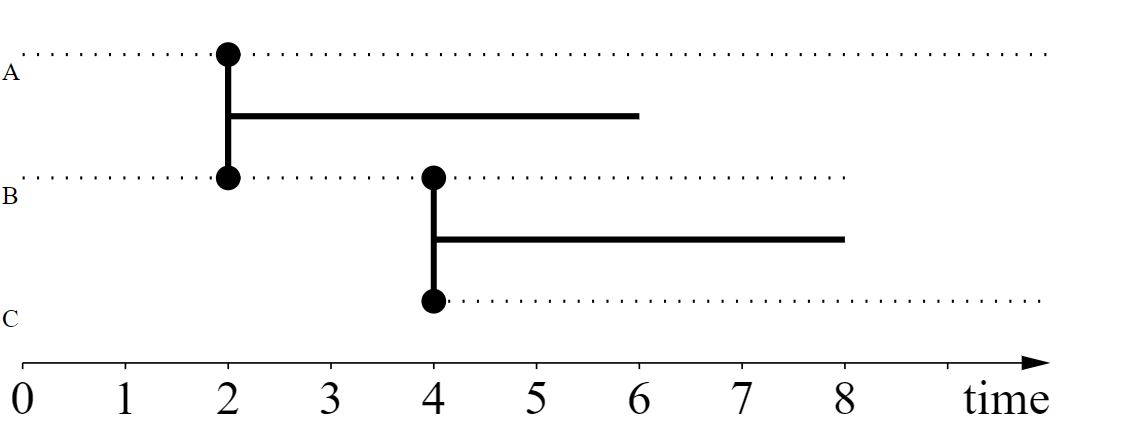
\includegraphics[width=0.5\textwidth]{exStreamGraph.JPG}
\caption{\textbf{Exemple de \stg{}} Dans cet exemple, on représente les interactions entre des animaux durant une expérience de 10 heures ($T=[0,10]$). Les nœuds sont les trois individus ($V=($A,B,C$)$) et leurs intervalles d'existence sont les suivants $T_{\text{C}}=[4,10], T_{\text{A}}=[0,10], T_{\text{B}}=[0,8]$, ils représentent les moments où les individus étaient présents dans le milieu d'observation. Enfin les liens $V=([2,6]\times (\text{A},\text{B})) \cup ([4,8]\times(\text{B},\text{C}))$ représentent les moments où les individus ont interagi.}
\label{exstreamgraph}
\end{figure}




\subsubsection{Quelques définitions}

Dans l'article \cite{stream}, de nombreuses notions sont ensuite définies de telle sorte à ce que dans le cas où le \stg{} serait statique, on retrouve les mêmes notions que pour un graphe classique.

Nous les évoquerons en temps voulu quand nous nous en servirons pour créer nos propres définitions.

\subsubsection{De l'intérêt de l'usage des \stgs{}}
La notion de \stg{} est très récente (2017)\cite{stream} et ce n'est évidemment pas la première tentative de formalisme pour des graphes dynamiques.

Par exemple on peut citer la représentation souvent utilisée en recherche opérationnelle, en "snapshot". Le nombre de noeuds d'un système est multiplié par un nombre de pas de temps discrets $n=\frac{t}{T}$. On crée ensuite un graphe temporel dont les noeuds sont étiquetés $(v,t_i)$, $v$ étant les noeuds et $t_i$ les temps auxquels ils sont considérés. Les liens peuvent être présents entre différents noeuds du même pas de temps, et on ajoute à cela une arête entre tous les couples de noeuds de la forme $(v,t_i),(v,t_{i+1})$. 
Dans ces cas-là les liens sont très souvent orientés pour indiquer le sens du temps. Ces graphes sont utilisés pour des calculs de flots optimaux \cite{map}. On peut d'ailleurs raccrocher cette représentation à la théorie des graphes multicouches, chaque couche correspondant à un pas de temps.

La notion de \stg{} permet de "se libérer" de la vision discrétisée des snapshots. Même si dans l'absolu, les deux visions permettent de stocker les mêmes informations et de faire les mêmes choses (il suffit pour cela de choisir un pas de discrétisation assez petit), la vision \stg{} permet d'aborder le problème sous un autre angle, plus orienté sur l'étude des interactions elles-mêmes.

\begin{figure}
\centering
	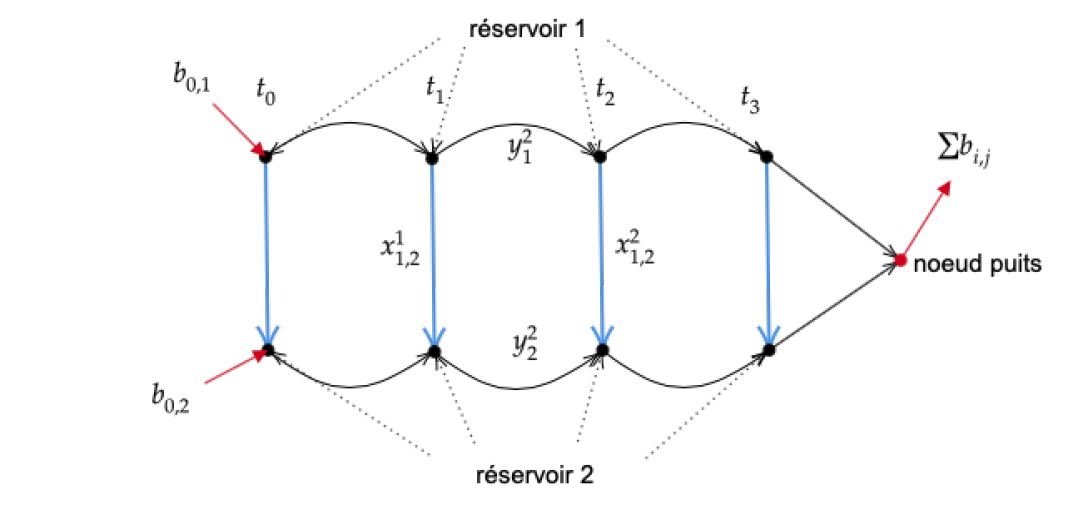
\includegraphics[width=0.7\textwidth]{snapshot.JPG}
	\caption{\textbf{Exemple de snapshot:} Un "snapshot" représentant un barrage (liens bleus) entre deux réservoirs aux temps $t_0,t_1,t_2,t_3$, tiré d'un projet MAP552}
\end{figure}



%conclusion partielle : cohérence avec les graphes classiques, à l'utilisateur de choisir ce qu'il veut obtenir

 
\section{Présentation d'un nouvel objet: le \stgm{}}



\subsection{Motivations}
\subsection{Définition}

\begin{defn}[\textbf{\Stgm}]
    
    Soit $T$ un intervalle de temps, ${\cal L}$ une structure de couches définie comme dans le cadre des graphes multicouches, et $V$ un ensemble de noeuds. 
    
    $T_M$ est un ensemble d'intervalles inclus dans $T$, indexé par les couches de $L$ et représente le temps d'existence de ces couches, avec pour contrainte que $\cup_{\alpha \in L} T_{\alpha} = T$ . $W_M$ est un sous ensemble de $T \times V \times L$, et contient les temps d'existence de chaque nœud couche, sachant que le temps d'existence d'un nœud-couche est forcément inclus dans le temps d'existence de la couche. Enfin, $E_M \subseteq T \times V \times L \times V \times L$ donne les liens entre les nœuds couches et leurs temps d'existence, sachant qu'un lien ne peut exister que pendant l'intersection des temps d'existence des nœuds-couches qu'il relie.
    
    L'objet $S_M = (T,T_M,V,W_M,E_M,{\cal L})$ est alors appelé \textbf{\stgm } (ou multilayer stream graph en anglais).
    
    On définit également les temps d'existence des noeuds-couches $T_{u,\alpha}$ et les temps d'existence des liens $T_{(u,\alpha),(v,\beta)}$ qui sont des unions d'intervalles.
	\end{defn}
	
	\begin{figure}[H]
		\centering
		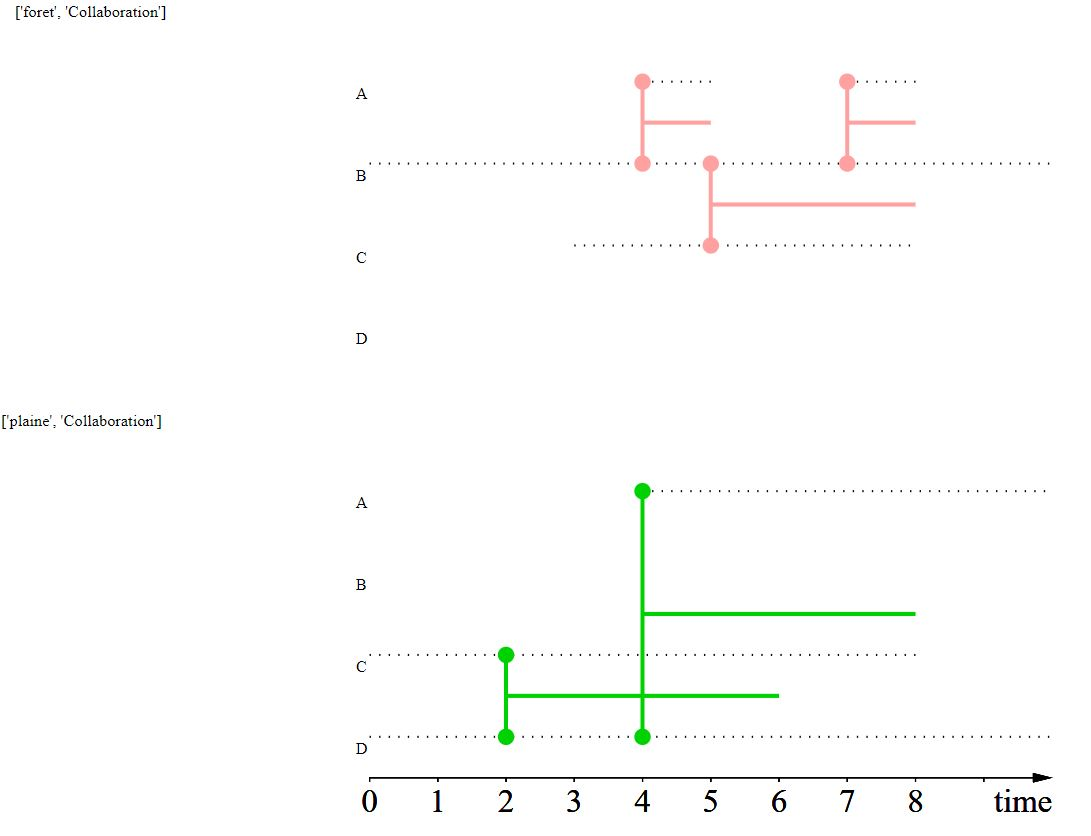
\includegraphics[width=0.8\textwidth]{exMultiStream.JPG}
		\caption{La représentation en \stgm{} des couches \texttt{["plaine","Collaboration"]} et \texttt{["foret","Collaboration"]}, générée avec "multiplex-stream" (description du programme en \cref{descode})}
		\label{exstgm}
	\end{figure}
	
	\begin{rmq}
		On peut s'interroger sur le bien-fondé d'utiliser l'objet \stg{} pour rajouter l'aspect temporel aux graphes multicouches. En effet, dans \cite{mlkiv}, les auteurs évoquent l'idée d'un aspect "continu", pouvant représenter le temps. Mais cette idée ne semble pas avoir été beaucoup exploitée, car les outils développés pour manipuler les graphes multicouches sont principalement matriciels et donc faits pour traiter un nombre de couches fini. De plus, des outils ont été spécifiquement créés pour traiter les \stgs{} et l'idée ici est de les exploiter.
	
	\end{rmq}

\subsection{Extraction de sous-graphes}
\label{sousgraphes}
\subsubsection{Projection par rapport au temps}
	Nous définissons ici deux moyens d'extraire des graphes multicouches en s'affranchissant du temps.
	
	Le premier est de \og prendre une photo \fg{} au temps $t$ :
	\begin{defn}[Graphe multicouche au temps t]
   	Le {\em graphe multicouche au temps t} $M_t$ s'écrit $M_t = (V_{M,t}, E_{M,t},V,{\cal L})$ avec $V_{M,t}$ et $E_{M,t}$ contenant les noeuds-couches et les arrêtes apparaissant au temps $t$.
   	$$ V_{M,t} = \{ (u,\alpha) | (t,u,\alpha) \in W_M\} $$
   	$$ E_{M,t} = \{(u,\alpha,v,\beta) | (t,u,\alpha,v,\beta) \in E_M\}$$

   \end{defn}

	\begin{figure}[H]
		\begin{minipage}{0.45\linewidth}
			\captionsetup{margin=10pt}
			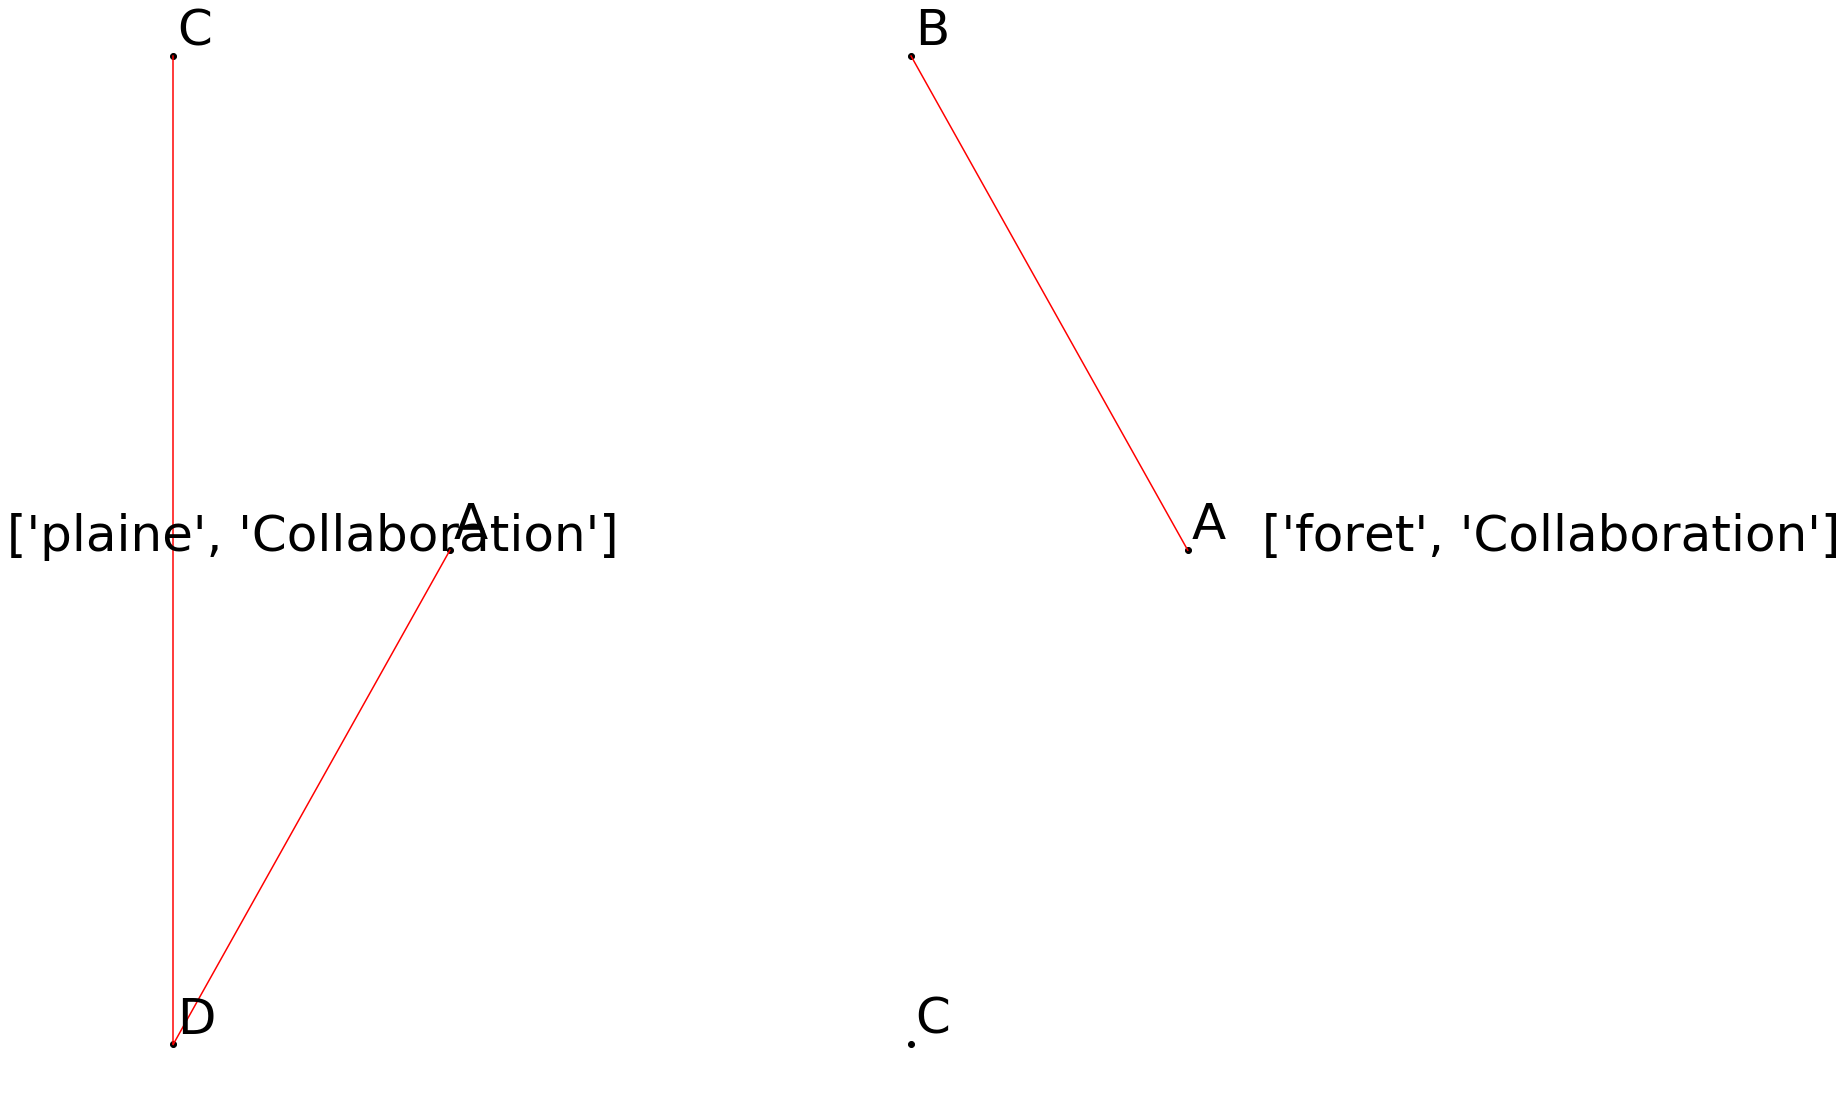
\includegraphics[width=\textwidth]{extrt4ex.png}
			\caption{Extraction du \stgm{} \ref{exstgm} au temps $t=4$}
		\end{minipage}
		\begin{minipage}{0.45\linewidth}
			\captionsetup{margin=10pt}
			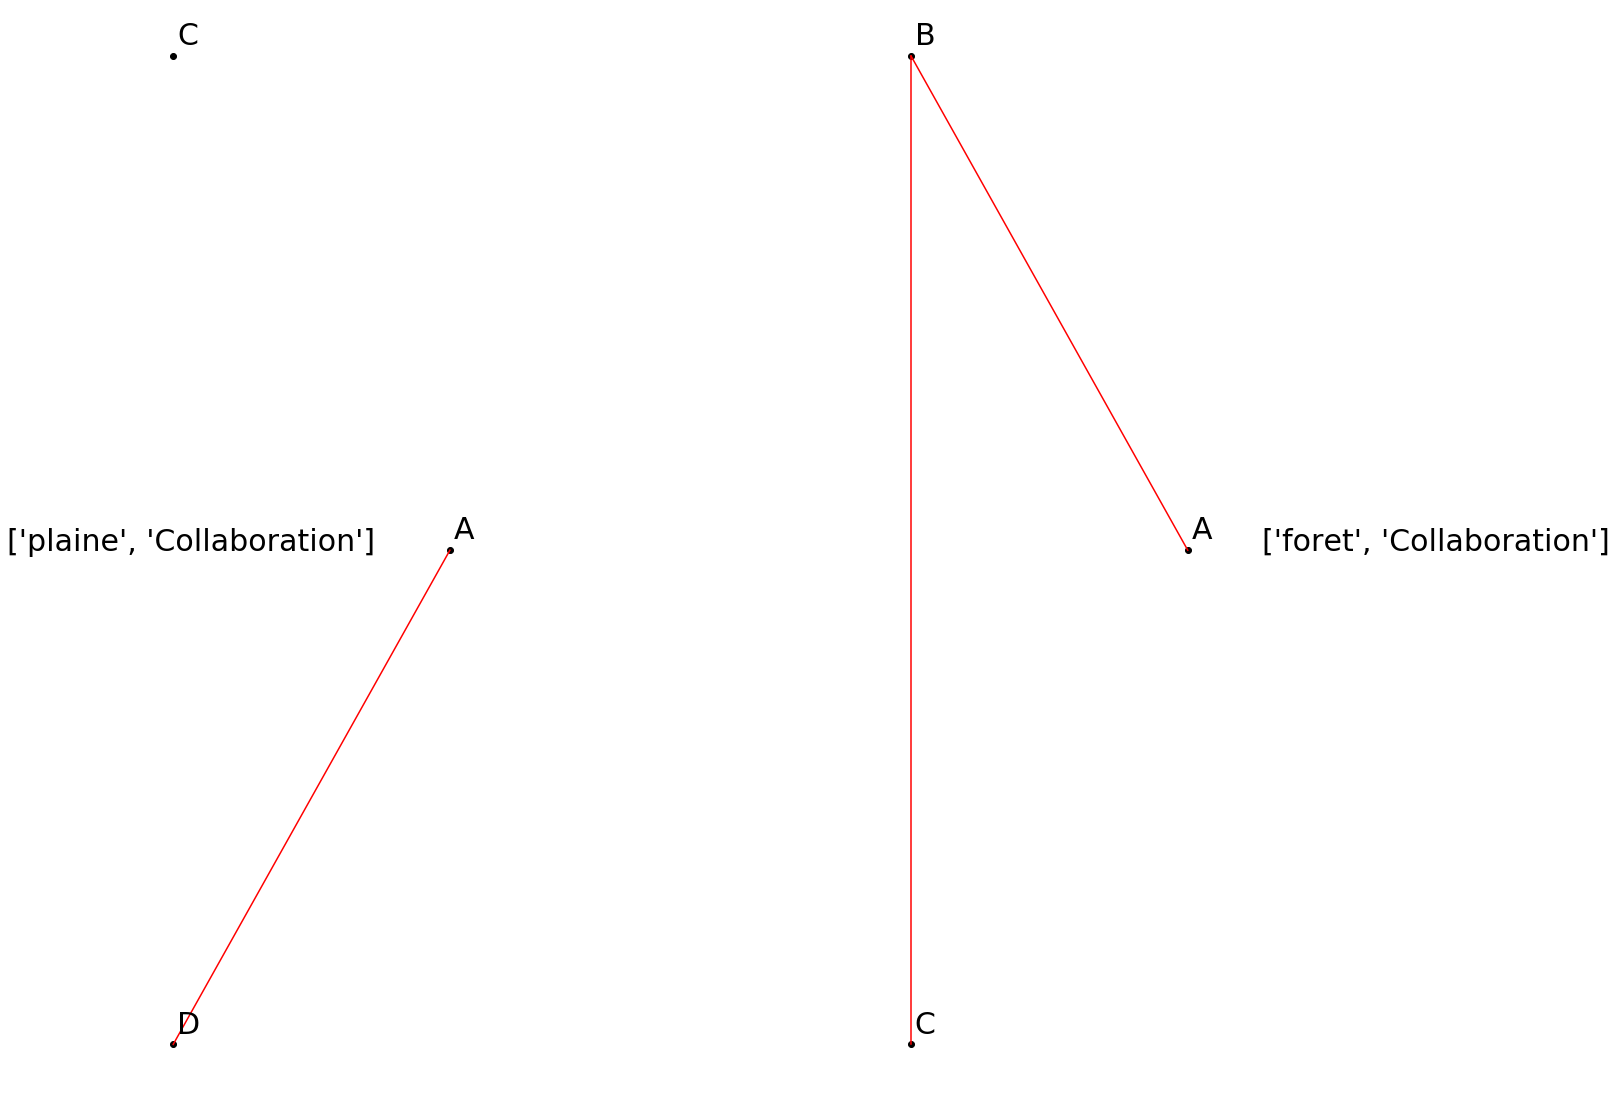
\includegraphics[width=\textwidth]{extrt7ex.png}
			\caption{Extraction du \stgm{} \ref{exstgm} au temps $t=7$}
		\end{minipage}
		\caption{dessin d'une extraction}
	\end{figure}

    Le second consiste à \og enregistrer \fg{} toutes les interactions pendant un laps de temps.
    \begin{defn}
    Le {\em graphe multicouche induit} $M_I(S_M) = (V_{M,I}, E_{M,I}, V,L)$ de $S_M$ est le graphe multicouche qui rassemble toutes les couches, noeuds couches et noeuds qui ont apparu durant $T$.
    \begin{align*}
    	V_{M,I} = \bigcup_{t\in T} V_{M,t}\\
    	E_{M,I} = \bigcup_{t\in T} E_{M,t}\\
    \end{align*}
    \end{defn}
    
    \begin{figure}[H]
    	\centering
    	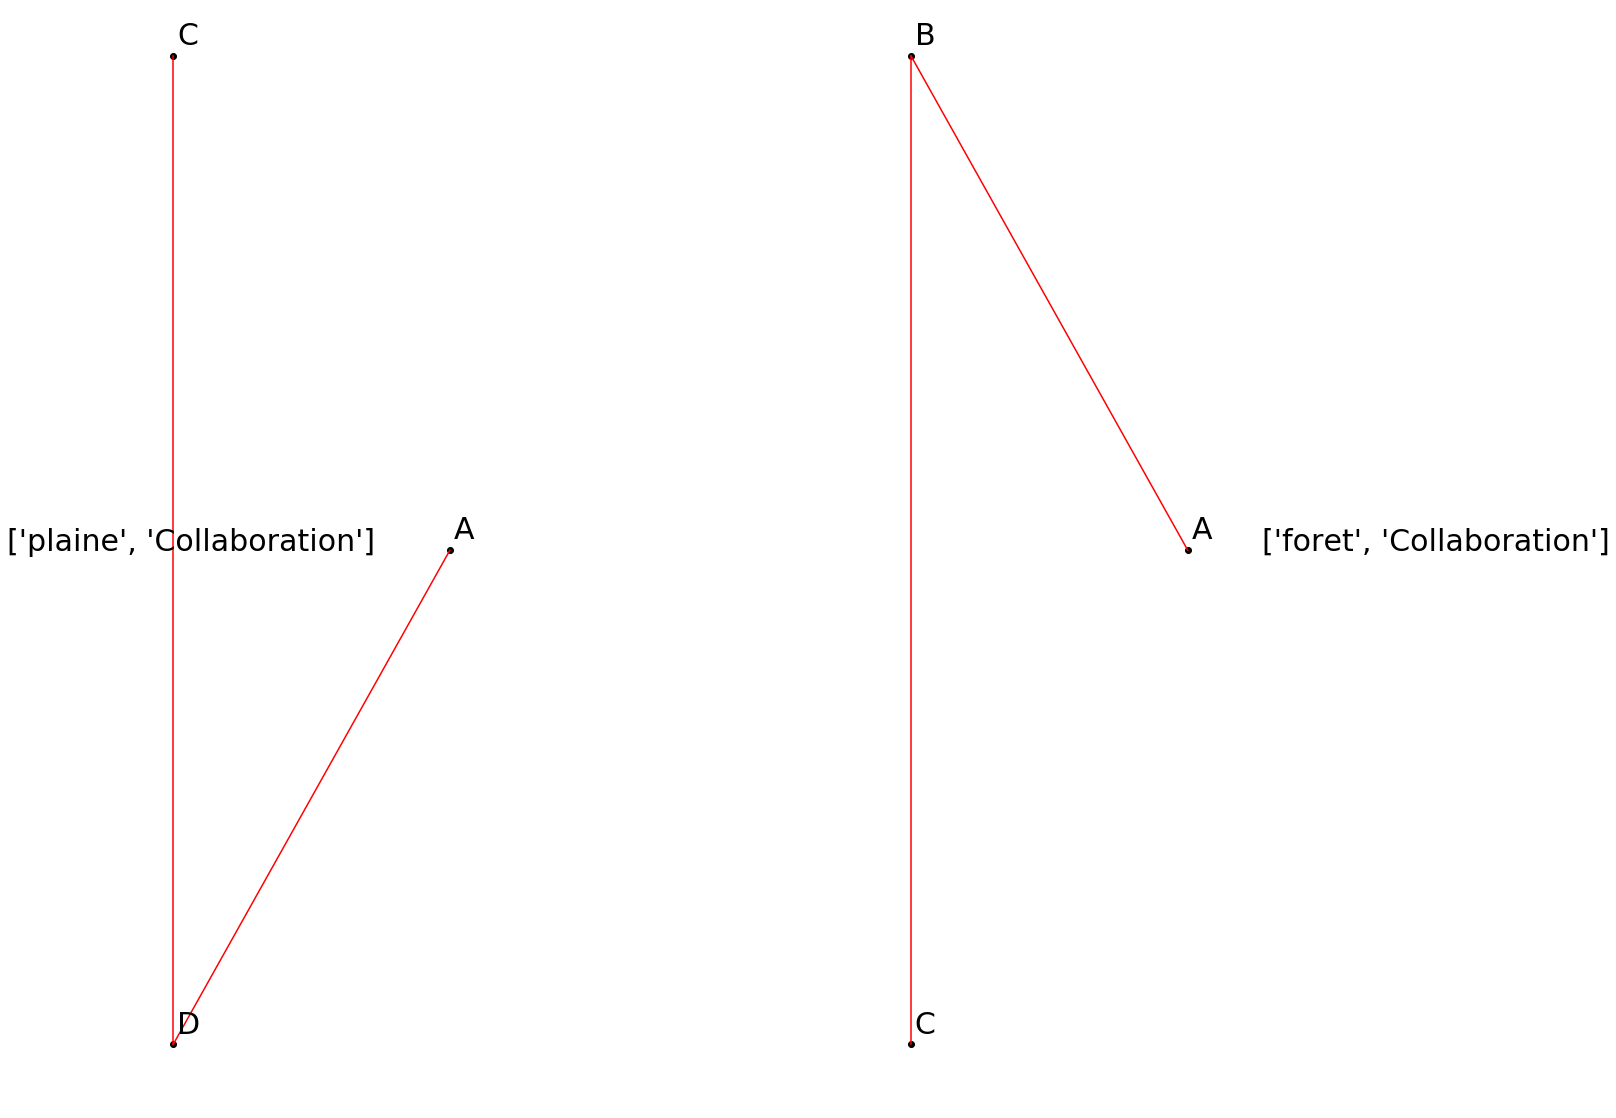
\includegraphics[width=0.5\textwidth]{extrt010.png}
    	\caption{Graphe multicouche induit du \stgm{} \ref{exstgm}.}
    \end{figure}
	


\subsubsection{Projection à partir de couches}
Comme dans \cite{mlkiv} pour les graphes multicouches, nous pouvons "classifier" les arêtes en plusieurs catégories :
	
	\begin{defn}[Arêtes de couplage, arêtes intra-couches et inter-couches]

   	Les {\em arêtes de couplage} sont définies par l'ensemble $E_C=\{(t,u,\alpha,v,\beta)\in E_M | u=v\}$.

    Les {\em arêtes intra-couches} sont définies par l'ensemble $E_I = \{(t,u,\alpha,v,\beta) \in E_M | \alpha = \beta \}$

    Les {\em arêtes inter-couches} sont définies par l'ensemble $\bar{E_I} = E_M\backslash E_I$.
    
	%(See fig.\ref{exIntraInter} for a visual representation.)
	
	\end{defn}	
	
	\begin{figure}[h]
		\centering
		%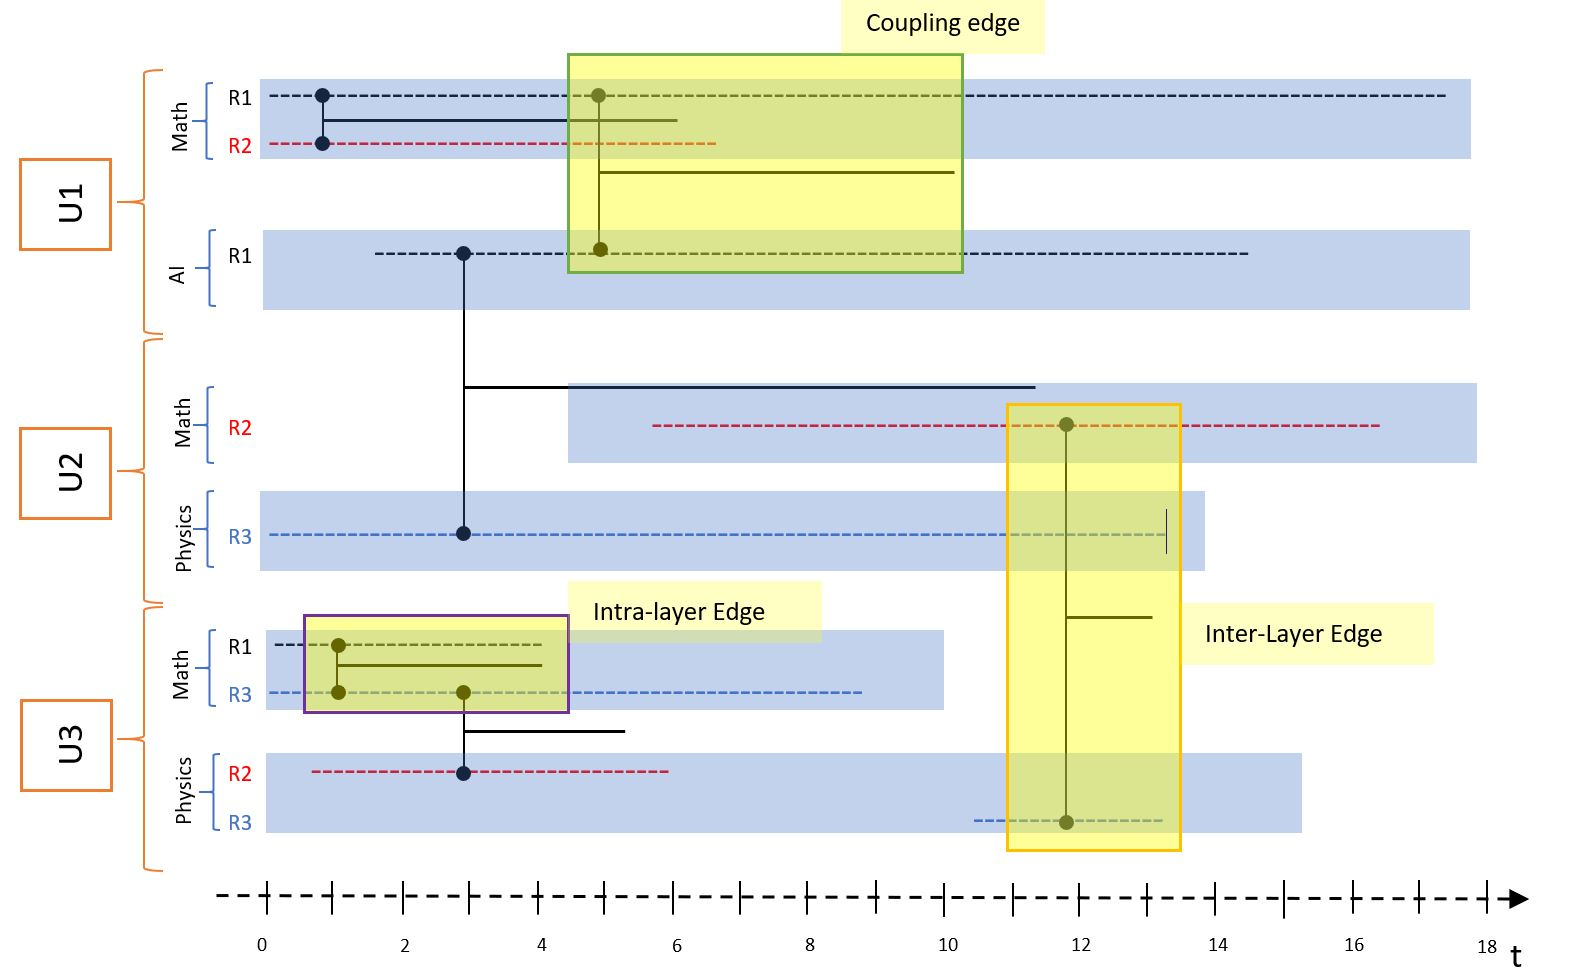
\includegraphics[width=\textwidth]{schemas/edgesCat.jpg}
		\caption{Illustration with our example of coupling edges, intra-layer edges and inter-layer edges}
		\label{exIntraInter}
	\end{figure}
	
	
	Comme dit précédement, les graphes multiplexes sont présents dans beaucoup de cas concrets et font l'objet d'études qui leur sont particulièrement dédiées. Nous définissons ici de façon formelle les \stgs{} multiplexes.
	
	\begin{defn}[\Stgs{} multiplexe]	
	Un {\em \stg{} multiplexe} est un graphe dans lequel chaque arête est une arête intra-couche ou une arête de couplage.
	\end{defn}
	
	Il peut être intéressant d'extraire certaines couches du \stgm{}, ou au contraire de se focaliser sur des interactions entre couches.
	 
	\begin{defn}[\Stg{} intra-couche]
	Pour chaque couche $\alpha \in L_1 \times \dots \times L_d$, le {\em \stg{} intra-couche} $S^{\alpha}$ est le \stg{} $S^{\alpha}=(T^{\alpha},V^{\alpha},W^{\alpha},E^{\alpha})$ tel que $T^{\alpha} = T_{\alpha} \in T_M$ est l'intervalle d'existence de $\alpha$. $V^{\alpha}$ est l'ensemble des nœuds couches dans la couche $\alpha$ et $W^{\alpha}$ représente leurs temps d'apparence dans la couche $\alpha$. $E^{\alpha}$ est le sous-ensemble $E_M$ contenant seulement les arêtes entre les noeuds-couches de $\alpha$.
	\end{defn}
	
	
	\begin{defn}[\Stg{} inter-couches]	
	Pour chaque doublet de couches $\alpha, \beta \in L_1\times \dots\times L_d$, le {\em \stg{} inter-couches} est le \stg{} $S^{(\alpha,\beta)} = (T, V^{\alpha,\beta},W^{\alpha,\beta},E^{\alpha,\beta})$ tel que : $T^{\alpha,\beta}=T^{\alpha}\cap T^{\beta}$ est l'intervalle durant lequel $\alpha$ et $\beta$ apparaissent simultanément. $V^{\alpha,\beta}$ sont tous les noeuds-couches du \stgm{} qui sont dans les couches $\alpha$ et $\beta$, $W^{\alpha,\beta}$ décrit leurs intervalles d'existence. Enfin, $E^{\alpha,\beta}$ sont les liens non orientés entre les noeuds couches des couches de $\alpha$ et $\beta$ avec leurs temps d'existence.
	\end{defn}
	
	%english Notice that for any layer $\alpha$,  is equivalent to $S^{(\alpha,\alpha)}$.

	On remarque que pour toute couche $\alpha$, $S^{(\alpha)}$ est équivalent à $S^{(\alpha,\alpha)}$.


	Après avoir extrait les \stg{} d'intérêt, il nous pouvons effectuer des opérations d'union et d'intersection pour trouver des propriétés intéressantes.
	
	\begin{defn}[Intersection de deux \stg{}]
	L'{\em intersection} de deux \stg{} $S_1$ et $S_2$ est un \stg{} et est définie de la façon suivante :
	\[
		S' = S_1 \cap S_2 = (T_1\cap T_2, V_1 \cap V_2, W_1 \cap W_2, E_1\cap E_2)
	\]
	\end{defn}
	

	\begin{defn}[Union de deux \stgs{}]
	L'{\em union} de deux \stgs{} $S_1$ et $S_2$ est un \stg{} et est définie de la façon suivante :
	\[
		S' = S_1 \cup S_2 = (T', V_1 \cup V_2, W_1 \cup W_2, E' \})
	\]
	$T'$ est un intervalle :
	\[
		T' = [\min(T_1,T_2),\max(T_1,T_2)]
	\]
	\[
		E' = E_1 \cup E_2 
	\]
	
	\end{defn}
	
	

	
	\begin{defn}[\Stg{} sous-jacent]
	Le {\em \stg{} sous-jacent} $S_U(S_M)$ de $S_M$ est $(T,V_M,W_M,E_M)$. C'est un \stg{} dans lequel les noeuds sont les noeuds-couches de $S_M$. Il peut être partitionné selon les différentes couches.
	\end{defn}
	
	\begin{defn}[\Stg aggrégé]
		Le {\em \stg{} aggrégé} $S_A(S_M)$ a le même intervalle d'étude $T$ que $S_M$. Ses noeuds sont les mêmes que ceux de $S_M$ et une arête existe entre deux noeuds de $S_A(S_M)$ si elle existe au même temps entre deux neouds-couches correspondants de $S_M$. 
	\end{defn}
	
	Nous pouvons à présent démontrer que le \stg{} sous-jacent est égal à l'union de tous les \stg{} inter et intra couches.
	
		
	\begin{prop}
		\[
			\bigcup_{(\alpha,\beta) \in L^2} S^{(\alpha,\beta)} = S_U(M_S)
		\]
	\end{prop}
	\begin{proof}
	On appelle $S=\bigcup_{(\alpha,\beta) \in L^2} S^{(\alpha,\beta)}=(T^{*},V^{*},W^{*},E^{*})$. Montrons que $S=S_U(M_S)= (T_U,V_U,W_U,E_U)$.
	
	$T=T_U$ par définition de $S_U$. Par construction des \stgms{}, pour tout $t$ dans $T$, il existe au moins une couche $\alpha$. Comme $T* = [\min_{\alpha \in L} (T^{\alpha}),max_{\alpha \in L} (T^{\alpha})]$, $t$ est forcément inclus dans $T*$. Chaque $T^{\alpha}$ est inclus dans $T$, donc $T^* \subseteq T$, donc $T^*=T_U=T$.
	
	$V_M = V_U$ par définition de $V_U$.$V^{*}=\bigcup_{(\alpha,\beta) \in L^2} V^{\alpha,\beta} \subseteq V_M$. Tous les noeuds de toutes les couches sont inclues dans $\bigcup_{(\alpha) \in L^2} V^{\alpha,\alpha} \subseteq V^{*}$, on obtient donc l'égalité $V_M=V_U=V^*$.
	Avec le même raisonnement, nous trouvons $W_M=W_U=W^*$.
	
	$E_U=E_M$ et $E^{*}=\bigcup_{\alpha,\beta \in L^2}(E^{\alpha,\beta})$ par définition. Comme $E^{\alpha,\beta}$ est un sous-ensemble de $E_M$ pour chaque couple de couches $\alpha,\beta$, $E^{*} \subset E_M$. On sait egalement que pour toute arête $e =(t,u,\alpha,v,\beta) \in E_M$, $e$ appartient à $E^{\alpha,\beta}$. Donc $E_M=E^{*}$.


On a donc bien une égalité terme à terme entre tous les éléments de $S$ et de $S_U(M_S)$.					
	\end{proof}

\paragraph{Remarque sur les extractions}
Nous avons donc exhibé un certain nombre d'extractions que nous pourrons maintenant combiner pour obtenir des graphes, des \stg{} ou des graphes multiplexes, en fonction des résultats que nous voudrons obtenir.

\subsection{Mesures}


Nous avons créé des mesures permettant de mesurer la présence de liens et de nœuds dans les graphes. Nous voulions que ces mesures soient adaptées à l'objet spécifique que nous étudions (et qu'elles prennent en compte l'aspect multicouche et l'aspect temporel de façon simultanée), qu'elles aient des noms qui évoquent intuitivement ce qu'elles expriment et qu'elles soient une généralisation des notions utilisées pour les \stg{}, pour les graphes multicouches et pour les graphes.

	\subsubsection{Nombre de nœuds}
	Le {\em nombre de noeuds dans un graphe} $G=(V,E)$ est $|V|$ et le nombre d'arêtes est $|E|$.
	
	Le {\em nombre de noeuds dans un \stg{}} $S=(T,V,W,E)$ est défini dans \cite{stream} comme $\hat{N}^T_n=\frac{|W|}{|T|}=\sum_{v\in V} n_v$ (ce qui est en fait le nombre moyen de noeuds au cours du temps). $n_v$ est appelé {\em contribution de v} et est égal à $\hat{N}^T_v=\frac{|T_v|}{|T|}$. Remarquons bien qu'ici cette notion est différente {\em du nombre de noeuds dans} $|V|$, sauf quand le \stg{} $S$ est constant au cours du temps.
	\newline
	
	Dans les graphes multicouches, une telle notion n'a pas été définie explicitement.
	Nous avons donc défini le {\em nombre moyen de noeuds par couche} comme :
	\begin{align*}
		\hat{N}_n^L(M_l) = \frac{\text{nombre de noeud-couches}}{\text{nombre de couches}}=\frac{|V_M|}{|L|}
	\end{align*}	    
	Remarquons que dans le cas d'un monocouche, nous retrouvons le nombre de noeuds classique, ce qui signifie que nous pouvons choisir cette mesure comme une généralisation du {\em nombre de nœuds} dans un graphe, comme cela a été fait dans \cite{stream} pour les \stg{}.
		
	
	\begin{defn}[Contribution des couches]
	On définit la {\em contribution} d'une couche comme suit : $n_\alpha = \frac{|T_{\alpha}|}{|T|}$. Le {\em nombre de couche dans un \stgms{}} est la somme des contributions. $\hat{N}^T_l = \sum_{\alpha \in L}\frac{ |T_{\alpha}|}{|T|}$.
    \end{defn}
	
	\begin{defn}[Contribution et quantité de nœud-couches]
	La {\em contribution d'un noeud-couche} dans un \stgm{} est $n_{v,\alpha} = \frac{|T_{v,\alpha}|}{|T|}$. Le {\em nombre de nœud-couches} est la somme de leurs contributions $\hat{N}^{T}_{nl}(M) = \underset{(u,\alpha)\in V_M}{\sum} n_{(u,\alpha)} = \frac{|W_M|}{|T|}$.
    \end{defn}
	
	Dans le cas d'un \stg{} monocouche, nous retrouvons bien que le nombre de noeuds est égal au nombre de noeuds-couches. En prenant le \stg{} sous-jacent du \stgm{}, on retrouve également que le nombre de noeuds est égal au nombre de noeuds couches. Nous avons donc là une généralisation satisfaisante du nombre de noeuds-couches.
    
   Enfin, nous définissons le \textbf{nombre de noeuds dans un \stgm{}} de la façon suivante : 
    
    \begin{defn}[Contribution et nombre de noeuds dans un \stgm{}]
    La {\em contribution} d'un noeud décrit le taux d'apparition d'un noeud dans les couches : $n_v = \frac{\sum_{\alpha \in L}|T_{v,\alpha}|}{\sum_{\alpha \in L} |T_{\alpha}|}$.
    
    Le {\em nombre de noeuds} est la somme de ces contributions :
    \begin{align}
    \hat{N}^{L,T}_n(M) = \sum_{v\in V} n_v= \sum_{v\in V} \frac{\sum_{\alpha \in L}|T_{v,\alpha}|}{\sum_{\alpha \in L} |T_{\alpha}|} 
    \label{numberNodes}
	\end{align}     
	
	\end{defn}
	
	Cette définition est cohérente avec les notions des multicouches et des \stg{} : si le noeud apparait dans toutes les couches tout le temps, nous trouvons $n_v=1$ comme dans les multicouches. Si tous les temps d'existence sont égaux, on retrouve $$n_v=\frac{\text{nombre de noeud-couches issus de v}\times |T|}{\text{nombre de couches}\times |T|}$$ Cette définition est donc une bonne généralisation pour tous les concepts.

	


	\subsubsection{Uniformité et densité}
	
	Dans les \stgs{} \cite{stream}, {\em l'uniformité entre deux nœuds} $u$ et $v$ est le ratio $\Cup (u,v) = \frac{|T_u\cap T_v|}{|T_u \cup T_v|}$, c'est à dire la probabilité, prenant un temps $t$ dans $T_u$ ou $T_v$, que les deux nœuds $u$ et $v$ puissent être reliés entre eux. L'uniformité est définie comme le rapport de tous les temps de co-existence sur les temps d'existence : $
 \Cup(S)=\sum_{u,v \in V \otimes V}\frac{|T_u\cap T_v|}{|T_u\cup T_v|}
$
	
		
	{\em L'uniformité } de deux noeuds-couches $(u,\alpha)$ et $(v,\beta)$ est définie sur le même modèle :
	\begin{align*}
		\Cup((u,\alpha),(v,\beta))=\mathbb{P}( t \in T_{u,\alpha} \cap T_{v,\beta} | t \in T_{u,\alpha} \cup T_{u,\beta}) \\
		= \frac{|T_{u,\alpha}\cap T_{u,\beta}|}{|T_{u,\alpha}\cup T_{u,\beta}|}
	\end{align*}

	{\em Le chevauchement} de deux couches $\alpha$ et $\beta$ est également défini comme suit :
	\begin{align*}
		\cup(\alpha,\beta) = \frac{|T_{\alpha}\cap T_{\beta}|}{|T_{\alpha}\cup T_{\beta}|}
	\end{align*}

    L'{\em uniformité des noeuds-couches} mesure le taux d'apparition simultanée des noeuds-couches dans le \stgm{} :
    \[
    	\Cup(M) = \frac{\sum_{(u,\alpha),(v,\beta) \ V_M \otimes V_M}{|T_{(u,\alpha)} \cap T_{(v,\beta)}|}}{\sum_{(u,\alpha),(v,\beta) \ V_M \otimes V_M}{|T_{(u,\alpha)}\cup T_{(v,\beta)}|}}
    \]
	
	Cette définition peut être nuancée en considérant que selon la nature du \stgm{}, certains noeuds peuvent ou ne peuvent pas apparaître simultanément. En particulier, {\em l'uniformité dans un \stgm{}} est définie ainsi:	
	
	\[
    	\Cup(M) = \frac{1}{|L|}\sum_{\alpha \in L} \frac{\sum_{(u,\alpha),(v,\alpha) \ V_M \otimes V_M}{|T_{(u,\alpha)} \cap T_{(v,\alpha)}|}}{\sum_{(u,\alpha),(v,\alpha) \ V_M \otimes V_M}{|T_{(u,\alpha)}\cup T_{(v,\alpha)}|}}
    \]
    
    On ne prend en compte que les temps d'apparition intra-layer, et on moyenne selon le nombre de couche. 


	Quand $\Cup=1$, on dit que le \stg{} est uniforme (autrement dit, $T_v = T_u, \forall (u,v) \in V^2$).


    Après avoir mesuré "à quel point le \stgm{} peut être connecté" grâce à l'uniformité, nous allons mesurer à quel point il est effectivement connecté grâce à a notion de \textbf{densité}.
    
    Dans les graphes classiques (non pondérés et non directionnel), la {\em densité} est la probabilité, prenant deux noeuds au hasard dans le graphe, qu'une arête existe entre ces noeuds.
    
		\[
			d(G) = \frac{|E|}{|V\otimes V|} = \frac{2\times |E|}{|V|(|V|-1)}
		\]
	Dans les \stg{}, la notion définie dans \cite{stream} est la même , en prenant un temps aléatoire, et deux noeuds au hasard existant à ce temps. 	

		\begin{align*}
			\delta_s(G) = & \mathbb{P}((t,u,v)\in E| (t,u),(t,v) \in W) \\
			 =  & \frac{\sum_{uv \in V \otimes V}{|T_{uv}|}}{\sum_{uv \in V\otimes V}{|T_u\cap T_v|}}= \frac{\int_{t\in T}{|E_t|dt}}{\int_{t\in T}{|V_t\otimes V_t|dt}}
		\end{align*}
		
	Nous pouvons ensuite définir la densité dans les \stgm{}. Nous remarquons premièrement que la densité mesure le "taux de connectivité", et qu'une fois encore, en fonction du système étudié, la définition peut changer puisque nous voulons que le cas où la densité est égale à 1 corresponde au cas où on ne peut pas rajouter d'arêtes. 

\begin{defn}[Densité d'un \stgm{}]	
	Nous appelons  $C \in T \times V_M\times V_M$ l'ensemble des connections autorisées dans le \stgm{}. Si certaines connections sont \og automatiques\fg ou "sous-entendues" comme par exemple les connections de couplage, nous ne les comptons pas dans $C$ non plus pour que le cas où la densité soit nulle corresponde au cas où on ne peut pas retirer de lien.

	La {\em densité du \stgm{}} s'écrit alors : 
	\[
		\delta_M (M) 
		= \frac{\int_{t\in T}|E_M,t|}{\int_{t\in T}|C_t|} 
		= \frac{\sum_{(u,\alpha)(v,\beta) \in E_M}|T_{(u,\alpha)(v,\beta)}|}{|C|}
	\]
\end{defn}	
	
	Par exemple, dans un \stg{} multiplexe, les liens possibles sont les liens intra couches et les liens de couplage : $C=\{(t,u,\alpha),(t,v,\beta))| t\in T_{u,\alpha} \cap T_{u,\beta}, u=v \text{or} \alpha = \beta)\}$ :

	\[
		\delta_M (M) = 
		\frac{|E_M|}{|C|}= 
		\frac{\sum_{(u,\alpha)(v,\beta) \in (V_M \otimes V_M)} |T_{(u,\alpha)(v,\beta)}|}
		{\underbrace{(\sum_{\alpha \in L}\sum_{(u,v) \in V\otimes V}|T_{u,\alpha} \cap T_{v,\alpha}|)}_{\text{arêtes intra-couches}}+\underbrace{( \sum_{u \in V } \sum_{(\alpha,\beta) \in L \otimes L}|T_{u,\alpha}\cap T_{u,\beta}|)}_{\text{arêtes de couplage}}}
	\]


\paragraph{}
Nous avons donc présenté les bases mathématiques d'un nouvel objet, le \stgm{}, ayant pour but de représenter des interactions de différentes natures, entre différents acteurs, en fonction du temps. Les mesures de nombre de noeuds et de liens, d'uniformité et de densité permettent d'adapter des notions présentes dans les graphes à notre objet. Les outils d'extraction comme le graphe sous-jacent, le graphe aggrégé ou les sous \stg{} inter et intra couches permettent de \og retrouver \fg{} les graphes classiques auxquels nous sommes habitués.
	
\section{Application à des données concrètes}


Nous avons ensuite construit une bibliothèque Python \cite{github} pour mettre en application les notions théoriques que nous avons présentées.

Nous allons présenter cette bibliothèque ainsi que sa structure. Puis nous allons exhiber un jeu de données qui s'y prête et nous allons donner un exemple d'utilisation concret de la bibliothèque et des notions créées.


\subsection{Structure de données et organisation du code} 
\label{descode}

	La gestion des \stgms{} implique assez rapidement de gérer un grand nombre d'informations "imbriquées" : chaque couche contient des noeuds, qui apparaissent à des temps précis, ces noeud-couches sont reliés par des liens, eux-mêmes apparaissant à des temps précis...
	
	J'ai choisi de construire des classes python pour simplifier la gestion de telles données, et pour permettre de vérifier simplement que le \stgm{} reste cohérent quand on le modifie.
	
	
	
	\begin{figure}[H]
		\centering
		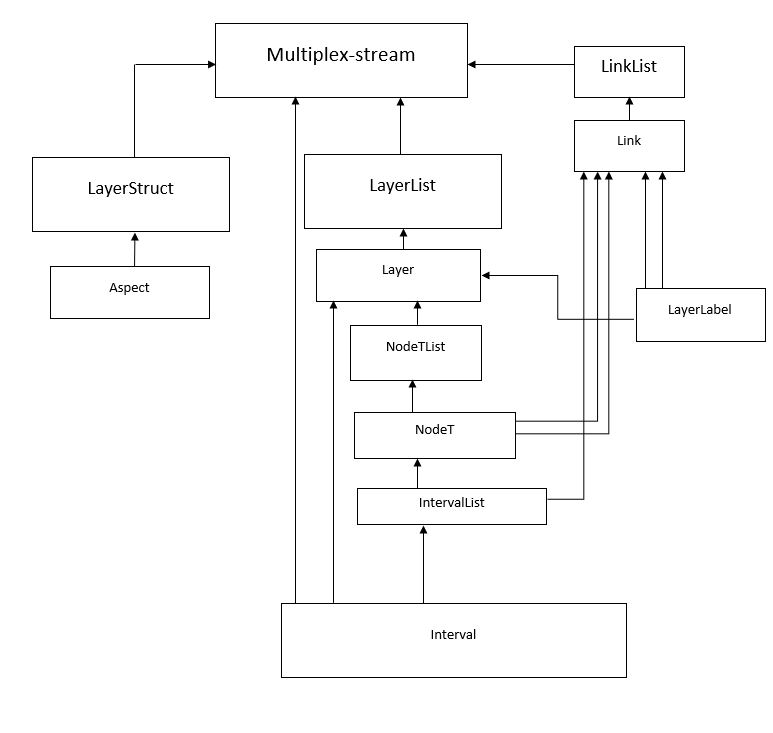
\includegraphics[width=0.5\textwidth]{codeStructure.JPG}
		\caption{Structure du code en classes }
	\end{figure}
	
	Toutes les listes sont toujours triées et les listes d'intervalles contiennent seulement des intervalles disjoints (quitte à fusionner certains intervalles).
	
	Dans un graphe simple, la {\em taille}, c'est à dire le nombre d'éléments à parcourir dans le graphe, est donnée par $c_G(G)=|V|+|E|$. Ici, nous avons choisi de stocker des couches, elles-mêmes contenant les noeuds-couches (et un intervalle), qui contiennent des listes d'intervalles. Les liens sont caractérisés par deux noeuds-couches et une liste d'intervalle.
	
	On appelle $n_I$ le nombre d'intervalle d'un ensemble, si celui-ci contient une liste d'intervalles.
	
	Ici la taille du \stgm{} est donc : $c_{MS}(M_S)=\sum_{e \in E_M} n_I(e) + \sum_{\alpha \in L} \sum_{v \in V} n_I((v,\alpha))$. Notons que dans le cas où le \stgm{} est statique et monocouche, on retrouve la taille d'un graphe classique.
	
	Pour traiter de graphes classiques, nous avons usuellement le choix entre utiliser une matrice d'adjacence (ce qui nous permet de savoir s'il existe un lien entre deux noeuds en temps 1) ou d'utiliser des listes d'adjacence (ce qui permet d'économiser de la mémoire).
	
	Ici, le stockage d'un lien est beaucoup plus coûteux puisqu'il faut stocker tous les intervalles d'existence, nous avons plutôt choisi d'utiliser une liste simple de tous les liens, mais stockés de façon ordonnés grâce à la bibliothèque \texttt{sorted collection}, pour laquelle tous les liens sont 
	

\subsection{CPGE : interactions entre élèves d'un même établissement}

    Nous avons en premier lieu testé notre logiciel avec une base de donnée de SocioPatterns (\cite{cpge}), recensant les interactions de "face à face" entre élèves (enregistrées toutes les 20 secondes grâce à des capteurs de proximité), leurs amitiés sur Facebook, et leur réponse à un questionnaire leur demandant s'ils étaient amis.

    Nous avons donc choisi une structure de couches suivante : \\
    {\tt L=[type de relation,classe,sexe]},\\
    avec\\
    {\tt type de relation = [face to face, facebook, contact, amitié]},\\
    {\tt classe = "MP","MP*1","MP*2","2BIO1","2BIO2","2BIO3","PSI*","PC","PC*"}.
  
    Le temps de prise a duré 5 jours, les détecteurs s'activant toutes les 20 secondes.
    
    Comme les seules interactions dépendantes du temps sont celles de face à face, on peut dire que le jeu de donnée donne lieu à un graphe "hybride". Nous avons considéré que les liens Facebook et d'amitié étaient donc constants au cours de l'expérience.
  
	\subsubsection{Représentation graphique}  
  
  Nous avons tout d'abord tenté de représenter le graphe multicouche en entier (\cref{lyceeentier}). La taille du jeu de données le rend difficile à représenter du fait que beaucoup de liens s'entrecroisent. (D'ailleurs, trouver un ordre optimal pour les noeuds qui limite les croisements des liens avec d'autres noeuds est un problème d'optimisation qui n'a pas encore été résolu de façon satisfaisante).
  
  Cependant, grâce à une coloration des liens intercouches, nous pouvons tout de même saisir la structure générale du jeu de données, ainsi que les pauses et les nuits.
	
	\begin{figure}[h]
	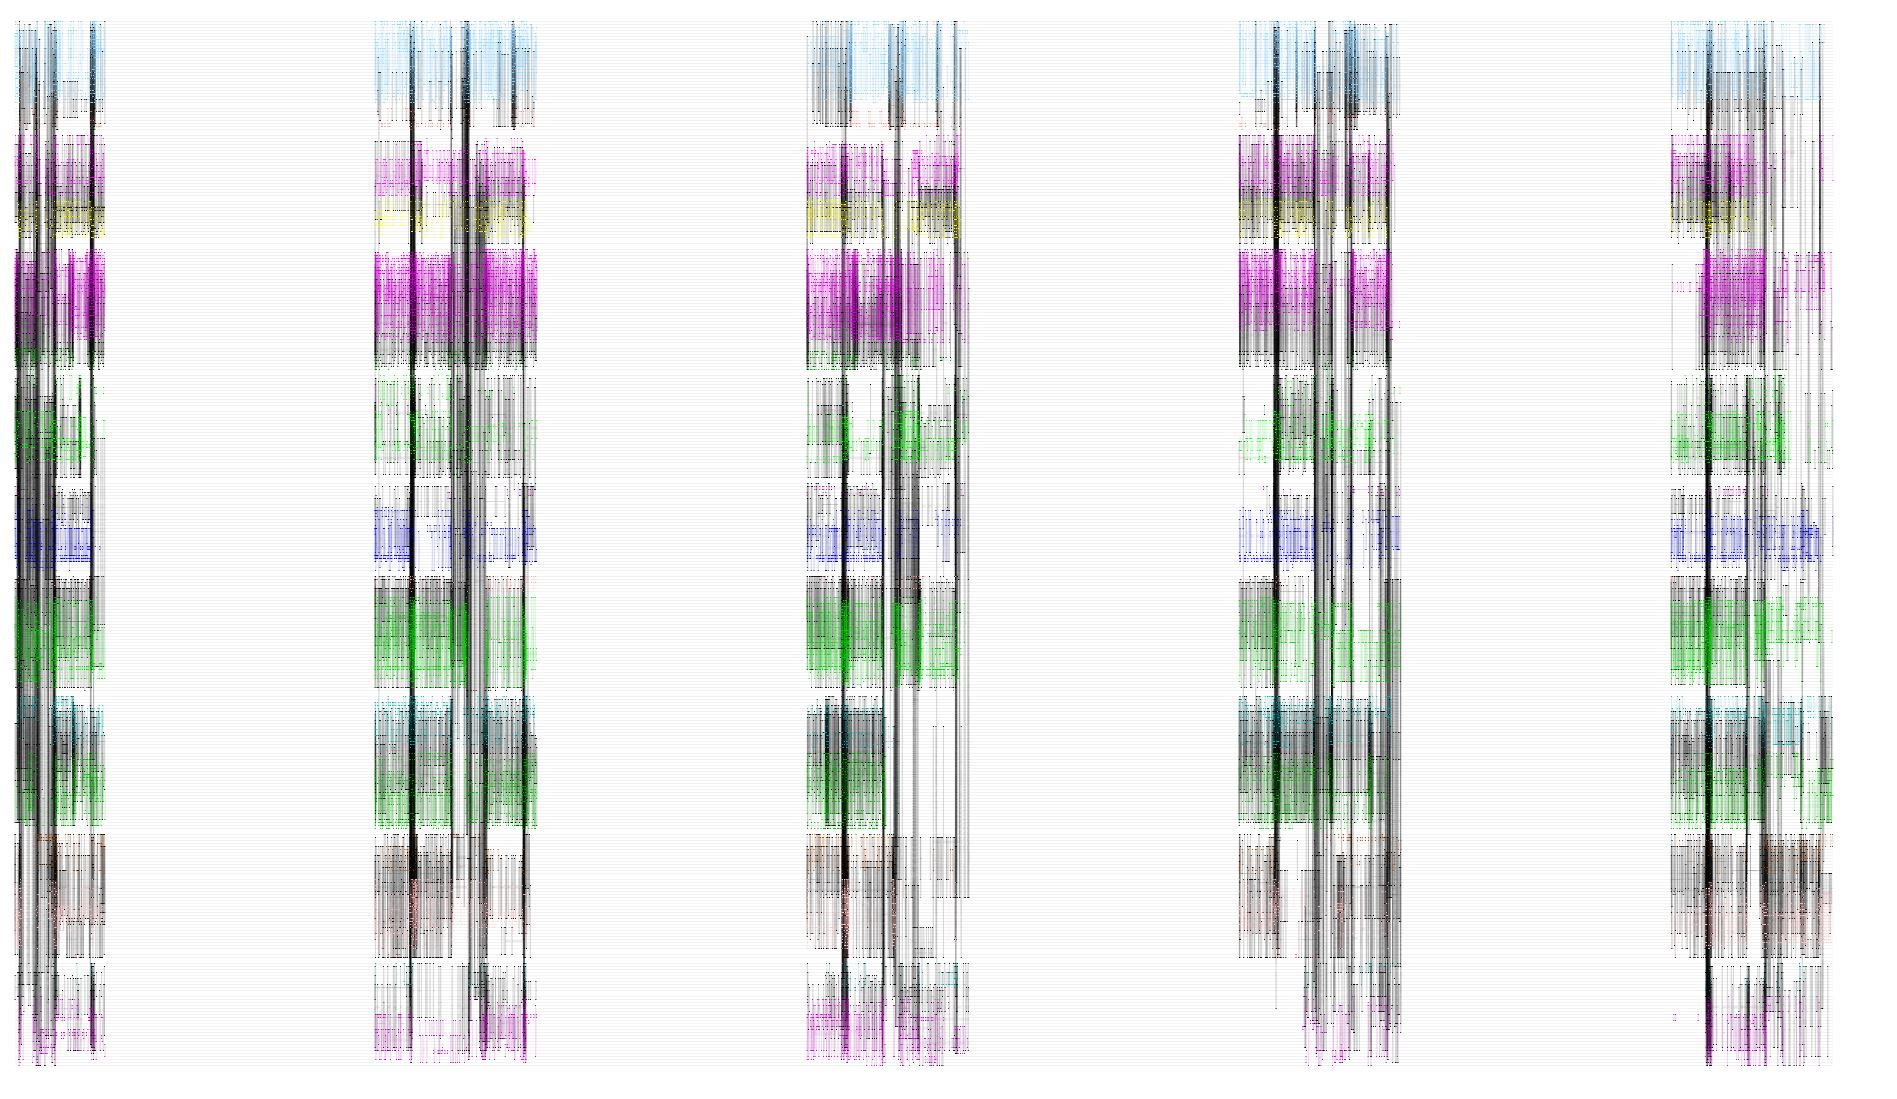
\includegraphics[width=\textwidth]{lyceeentier.JPG}
	\caption{\textbf{Visualisation du \stgm{} du dataset \cite{cpge}.} Les liens intra-couches ont été coloriés dans des couleurs aléatoires. On remarque des apparitions de liens inter-couches assez importants au moment des "pauses" (il y a visiblement une pause le matin, une autre le midi, et à la fin de la journée). On peut également visualiser simplement l'emploi du temps des élèves (représentés par des vides dans le graphe).}
	\label{lyceeentier}
\end{figure}





\subsubsection{Sous-graphes, sous \stg{} et sous graphes multicouches}

Voici quelques exemples de sous-graphes tels que nous les avons définis \cref{sousgraphes}. Nous avons décidé de nous cantonner aux relations \texttt{'face to face'} et \texttt{'facebook'}, mais ces résultats sont généralisables à plus de couches. 

\paragraph{Graphe multicouche induit}
	Le graphe multicouche induit des relations de deux classes, filles et garçons, est représenté \cref{completinduit}. Ici, chaque cercle correspond à une couche différente.
	
\begin{figure}[H]
	\centering
	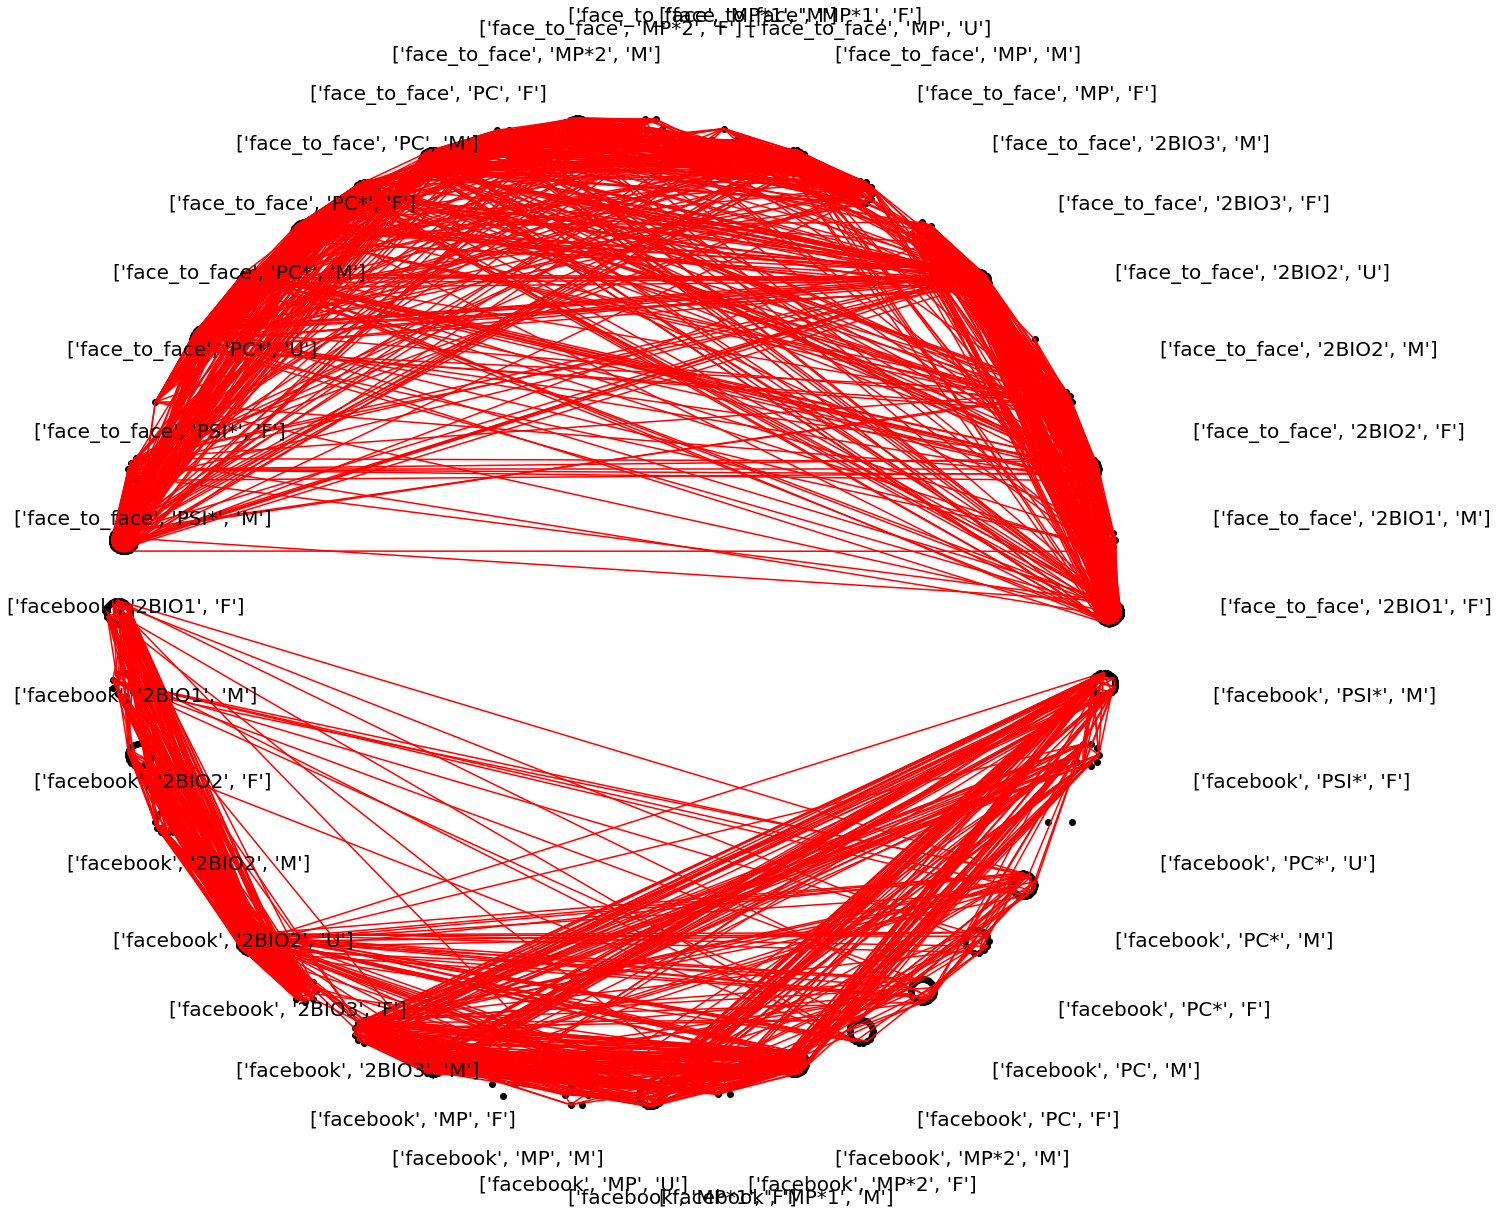
\includegraphics[width=0.5\textwidth]{tout.png}
	\caption{\textbf{Graphe induit}}
	\label{completinduit}
\end{figure}

	Nous représentons ensuite les sous-graphes multicouches intra-couches et inter-couches induits des couches de deux classes différentes pour plus de visibilité. \cref{induit}

\begin{figure}[H]
	\begin{minipage}[t]{0.48\textwidth}
		\captionsetup{margin=10pt}
		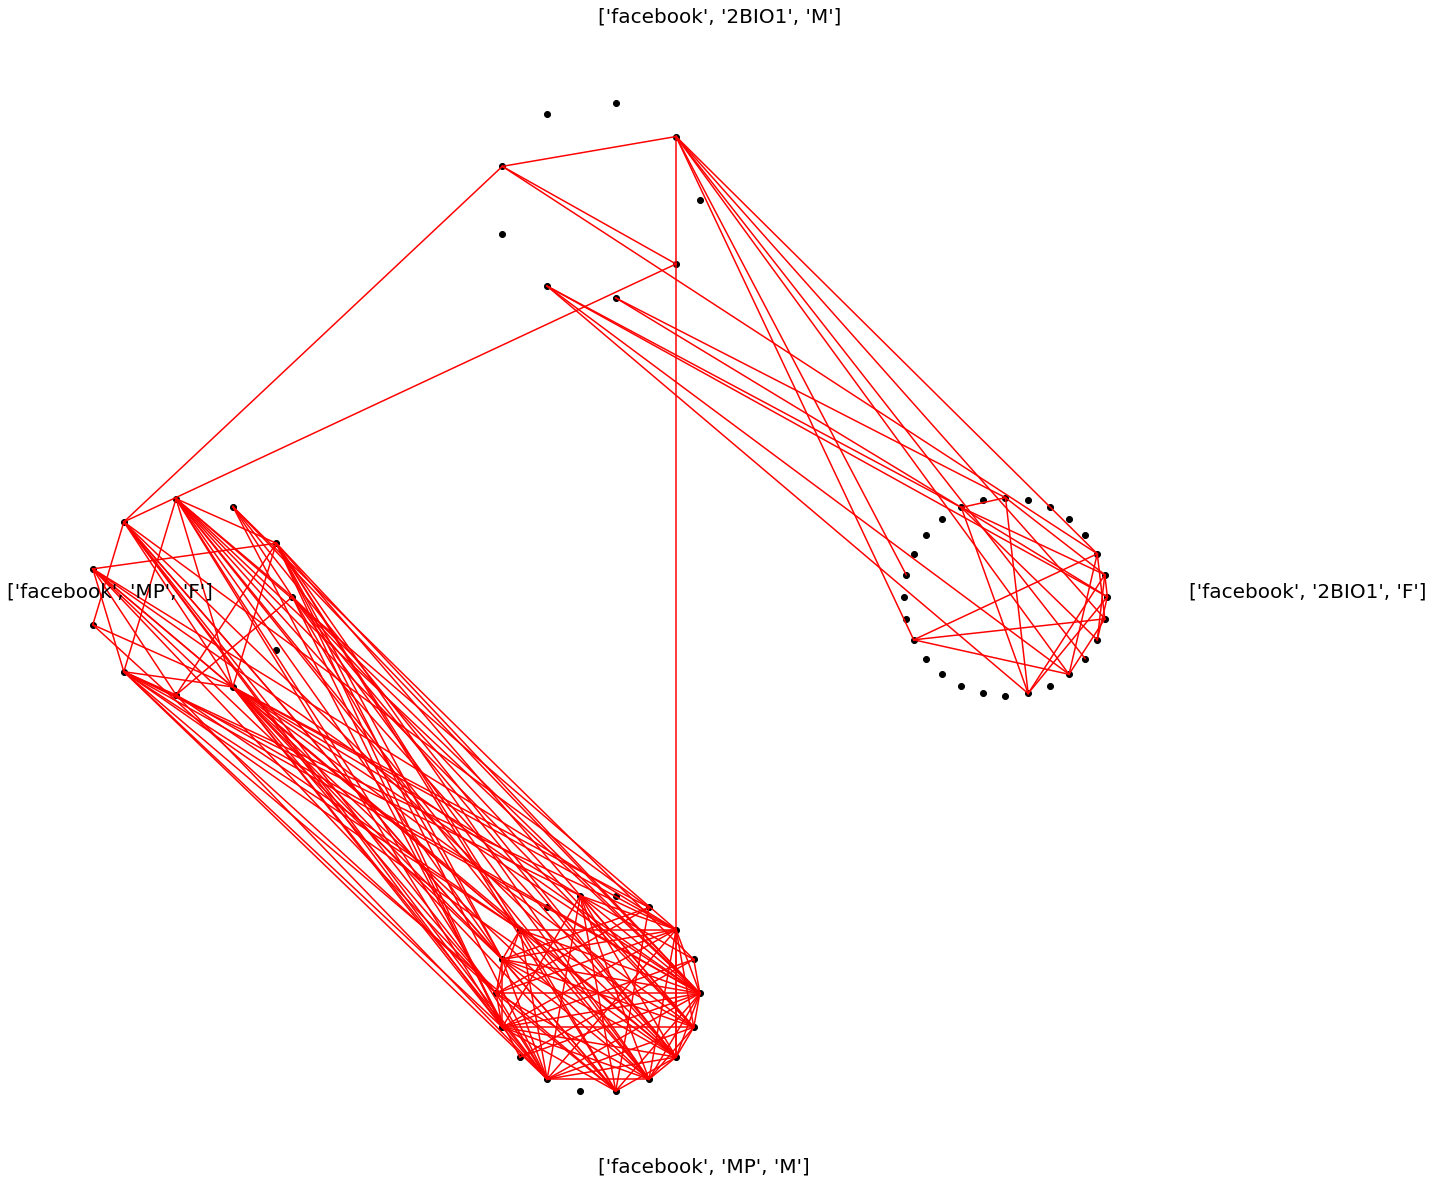
\includegraphics[width=\textwidth]{sousmulticlasse.png}
	\caption{\textbf{Visualisation du sous graphe multicouches des relations \texttt{'facebook'}, entre les élèves de deux classes} : les \texttt{'2BIO1'} et les \texttt{'MP'}.}
	\end{minipage}
	\begin{minipage}[t]{0.48\textwidth}
		\centering
		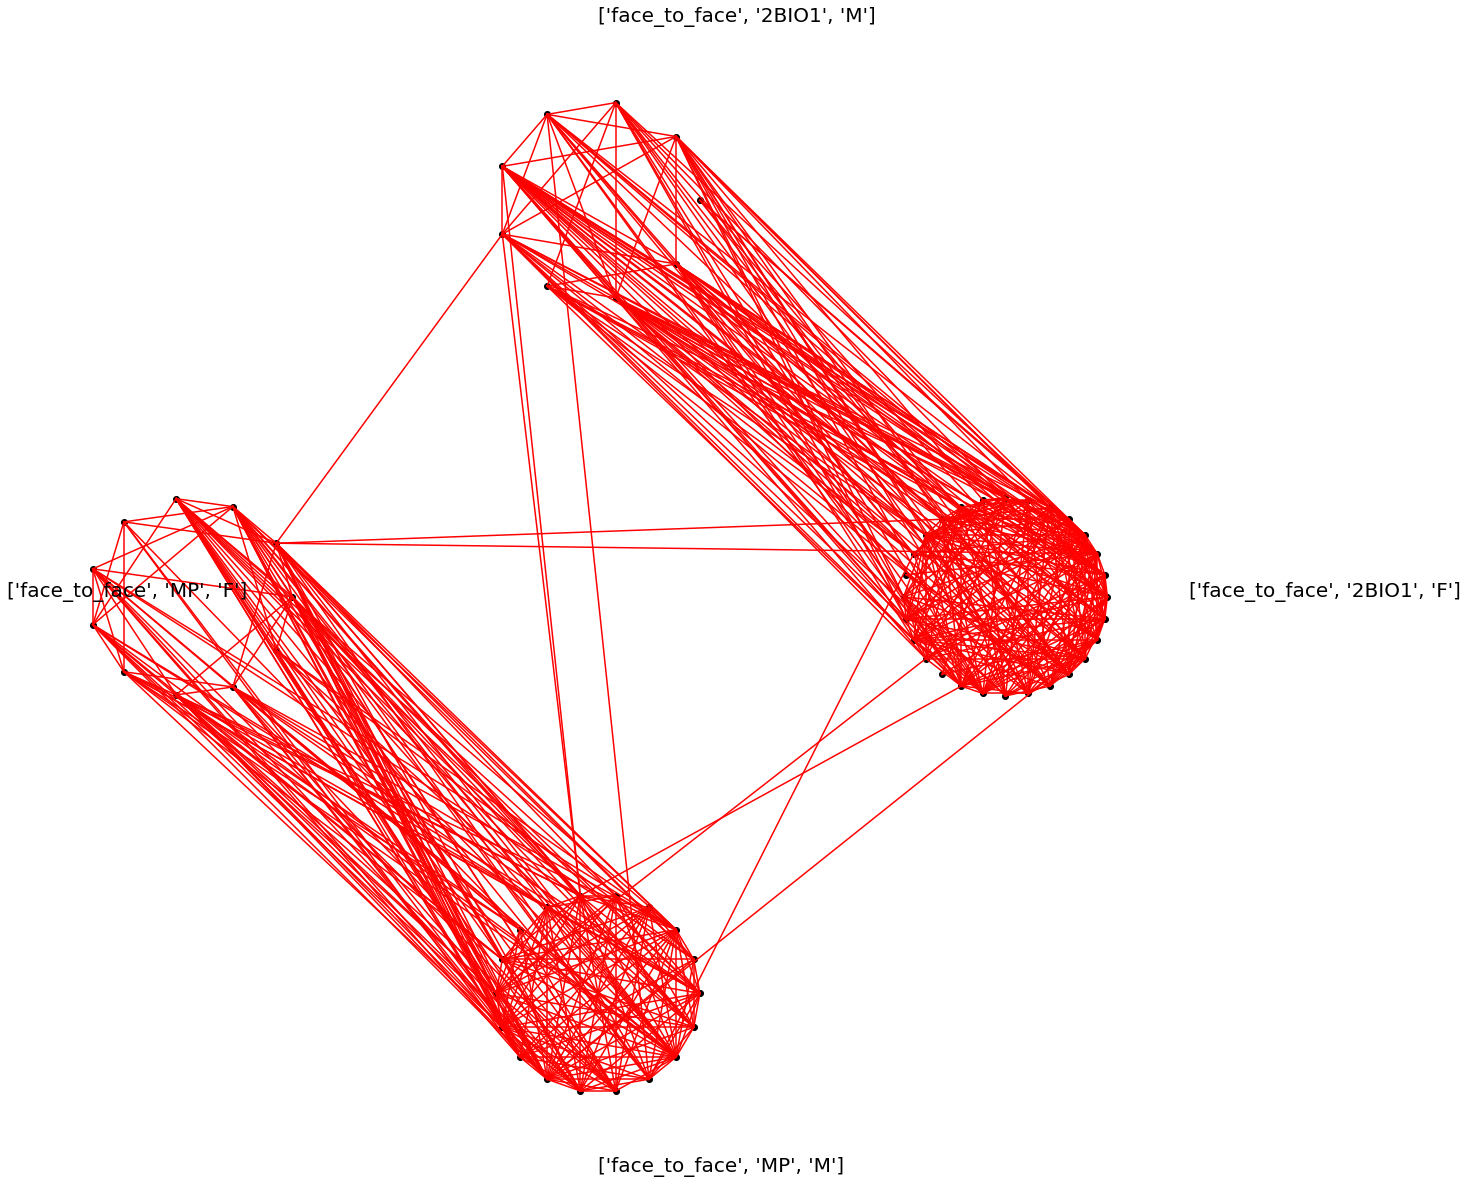
\includegraphics[width=\textwidth]{sousmulticlasseftf.png}
		\captionsetup{margin=10pt}
		\caption{\textbf{Visualisation du sous graphe multicouches induit des relations \texttt{'face to face'}, entre les élèves de deux classes} : les \texttt{'2BIO1'} et les \texttt{'MP'}.}
	\end{minipage}
	\caption{\textbf{Comparaison entre différents aspects du graphe multicouche. } On peut s'intéresser à la pertinence de séparer filles et garçons en différentes couches. En revanche, la séparation entre différentes classes semble être justifiée.}
	\label{induit}
\end{figure}
	
	
\subsubsection{Etude des densités intra-couches et inter-couches pour plusieurs aspects}
	On peut alors se demander en regardant ces interactions \cref{induit} et \cref{completinduit} , si le partitionnement différenciant les femmes et les hommes est "visible" d'un point de vue des interactions.

Nous avons donc calculé la densité des relations femmes/hommes comparée aux densité des relations au sein des hommes et des femmes, au fil des jours. Cette densité correspond à la probabilité, prenant un temps aléatoire et deux noeuds aléatoires, ces noeuds soient reliés par une arête.

Au sein des hommes, des femmes, ou pour la densité totale, on calcule donc :$$
\delta = \frac{\sum_{u,v \in V\otimes V} |T_{uv}|}{\sum_{u,v \in V \otimes V}|T_u\cap T_v|} = \frac{|E|}{|T|(|V|(|V|-1))}$$
et dans le graphe biparti des interactions hommes-femmes, la densité est :
$$\delta_{biparti}=\frac{\sum_{u,v \in V_f \times V_h} |T_{uv}|}{\sum_{u,v \in V_f \times V_h}|T_u\cap T_v|}=\frac{|E|}{|T||V_f||V_h|}$$
\begin{figure}[H]
	\centering
	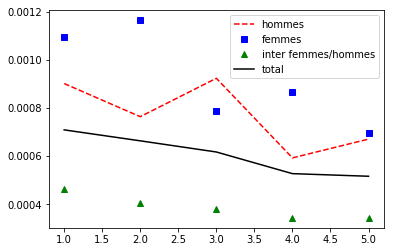
\includegraphics[width=0.5\textwidth]{compfg.png}
	\caption{Densité des relations au sein des femmes, des hommes, des relations inter-hommes/femmes, et des relations en général prise chaque jour de la semaine.}
	\label{densitesemaine}
\end{figure}

Nous voyons qu'une tendance se confirme : les relations sont plus denses au sein d'un même sexe qu'en moyenne, et les relations inter-sexes sont moins denses qu'en moyenne. La question que nous pouvons alors nous poser est "qu'est-ce que nous apporte la vision des \stgm{} ?" Nous avons donc tracé les mêmes densités pour des graphes multicouches sous-jacents correspondant aux jours de la semaine (\cref{dsj}). Nous obtenons les mêmes tendances mais moins "contrastées" puisqu'une relation de longue durée \og pèse \fg{} autant qu'une relation de courte durée qui a pu être enregistrée \og par hasard \fg{}, mais qui ne reflète pas une réelle interaction.

\begin{figure}[H]
	\centering
	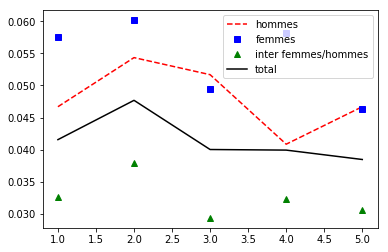
\includegraphics[width=0.5\textwidth]{densitesj.png}
	\caption{Densité des graphes sous-jacents pour les 5 jours de la semaine.}
	\label{dsj}
\end{figure}

Nous avons comparé les différentes densités pour les aspects \texttt{'facebook'} et \texttt{'frienship'}. Nous avons alors relevé les mêmes tendances, et même nettement plus accentuées pour les relations amicales, où les relations intra-hommes passent en dessous de la moyenne. \cref{comp}

\begin{figure}[H]
	\centering
	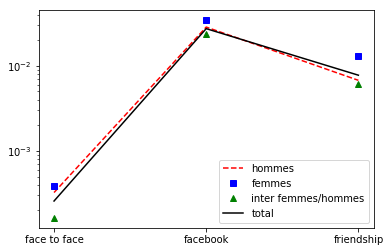
\includegraphics[width=0.5\textwidth]{comparatif.png}
	\caption{Comparatif des densités pour les relations \texttt{'face to face'}, \texttt{'facebook'} et \texttt{'friendship'} en échelle logarithmique, pour les aspects \texttt{'hommes'}, \texttt{'femmes'}, le graphe inter-couche \texttt{'hommes'/'femmes'} et le graphe en entier.}
	\label{comp}
\end{figure}  

Nous avons donc montré que les outils créés pour les \stgm{} peuvent servir pour analyser des interactions entre individus de façon plus nuancée. La densité associée aux sous-\stg{} inter-couches et intra-couches sert à caractériser des interactions de différents types entre plusieurs groupes d'individus.


\section{Conclusions et perspectives}

    Nous avons donc présenté notre nouvel objet ainsi que les raisons qui ont mené à sa création. Nous avons créé plusieurs notions pour nous permettre d'extraire des graphes d'intérêt et de prendre des mesures, et nous avons montré un exemple d'utilisation de ces notions grâce à un jeu de données.
    
    Pour la suite du stage, nous avons trouvé deux jeux de données très différents pouvant se prêter à notre étude, et permettant des applications diverses.
    Le premier rencense les personnages, dialogues et lieux des films StarWars, ainsi que leurs interactions dans le temps. Le but sera de "trouver" quels sont les personnages, sujets et lieux "principaux" ou "centraux", en adaptant des méthodes d'intrication \cite{intrication}, existantes pour les graphes multicouches, aux \stgm{}.
    Le second recense tous les vols sur le sol américain entre 1987 et aujourd'hui, pour différentes compagnies aériennes (représentant les différentes couches). Cette fois-ci, il nous faudra adapter le modèle de \stgm{} simple au même objet mais dans lequel les liens sont "instantanés" et coûtent un temps $\gamma$ à être parcourus. Le but sera ensuite d'étudier la "centralité" des aéroports ou des compagnies aériennes, grâce à des mesures multicouches, des simulations de trajets aléatoires et peut-être une adaptation du PageRanking à notre nouvel objet, en nous inspirant de \cite{centraliteMulti}.
    
    Bien que la notion de \stgms{} semble naturellement adaptée en théorie à de nombreux jeux de données, peu d'entre eux sont en fait accessibles à l'heure actuelle. En effet, le formalisme n'existant pas, il n'a probablement pas semblé utile de collecter autant d'informations dans un dataset que le type des relations et surtout les temps d'interaction. Mais avec le nombre croissant de "big datas" à notre disposition, il est très probable que nous ayons accès de plus en plus souvent à ce genre de données.

    \nocite{*}
    \bibliographystyle{plain}
	\bibliography{rapport}

\end{document}
